\chapter{Context of the study} % Optimizing the performance of a centrifugal pump with data assimilation

%– Le récit de l’expérience préprofessionnelle doit faire état de toutes les fonctions exercées par le stagiaire à son poste. Il doit comporter des développements techniques (illustrés par des schémas expliqués et commentés, par exemple), mais il s’agit avant tout de donner au lecteur une idée de ce que furent l’emploi du temps du stagiaire, ses tâches quotidiennes, les contraintes du métier, la nature des relations humaines dans cet environnement, les difficultés rencontrées et les résultats obtenus.
%– Les connaissances techniques acquises doivent transparaître dans le document. Le correcteur évaluera si celui-ci fait état d’une maîtrise réelle des outils (informatiques, mécaniques, etc.) utilisés pendant le stage. En outre, il estimera le niveau des connaissances techniques acquises que la rédaction du rapport aura su mettre en évidence.

% MIEUX INTRODUIRE PK CE STAGE, DA EXEMPLE MTO ETC -> Pa

The internship began in February 2025. I was provided with a fix computer, credentials to connect to the \ac{TGCC} (Irene - Skylake and Rome partitions) and Cassiopée supercomputers, and the link to the \ac{CONES}'s gitlab\footnote{\url{https://gitlab.ensam.eu/pe431/cones-dev}}. Marcello MELDI, Antoine DAZIN and Miguel MARTINEZ VALERO who are my internship supervisors, showed me around the lab.
Then, Tom MOUSSIE and Miguel MARTINEZ VALERO, my co-officies, explained me the basics of \ac{OpenFOAM} and CONES, the DA code. I was able to run a few tests on OpenFOAM on the supercomputers, which allowed me to familiarize myself with the tools and the code.

To introduce the topic of my internship, let’s start with a simple example: weather forecasting. Meteorologists improve predictions by combining numerical models with real-time observations through a process called data assimilation. This approach corrects model errors and leads to more reliable forecasts.

Similarly, in fluid mechanics, scientists rely on measurements and governing equations to study flow behaviour. While analytical solutions exist for simple cases, realistic flows often require numerical simulations. Unfortunately, high-fidelity simulations are too computationally demanding for most industrial applications.

To overcome this, simplified models with adjustable parameters are used. These parameters must be calibrated to specific flow conditions, typically using experimental data. For instance, techniques such as the \ac{IBM}, described later, adopt a global modelling strategy, even though the underlying flow physics can vary significantly at a local level. High-fidelity data are therefore essential for proper calibration.

Manual parameter tuning works when only a few variables are involved, but it quickly becomes inefficient and unreliable as the number of parameters grows. This is why mathematical approaches such as the EnKF are increasingly used—and this motivation led to the definition of my internship topic.



%To introduce the topic of my internship, let's take a simple example: the weather forecast. Meteorologists use data assimilation to improve weather predictions by combining numerical models with real-time observations. This process helps correct model errors and provides more accurate forecasts.
%To understand fluid behaviour, scientists can also rely on physical measurements and governing equations. While analytical solutions exist for simple cases, more complex flows require numerical simulations. However, high-fidelity simulations remain too computationally expensive for industrial use.
%This limitation has led to the development of approximate models involving tunable parameters. These parameters are calibrated for specific flow conditions, using experimental data. Techniques such as the \ac{IBM}, which will be detailed later, use a global approach, while the physics of the flow can locally be very different. That's why it relies on such high-fidelity data calibration.
%Manual tuning is feasible for a small number of parameters but becomes inefficient and inaccurate as complexity increases. This justifies the use of mathematical approaches like the EnKF, which motivated the definition of my internship topic.

%When scientists want to understand fluid behaviour, they can collect physical data through measurements. They can also rely on physical laws. In very simple cases, analytical solutions can be found. For more complex cases, these physical laws can be discretized to run numerical simulations.
%Today, thanks to numerical computation, we are able to simulate the behaviour of fluids. However, the computational cost of an "exact" fluid simulation is still too high to be used in industrial applications. This has led researchers to develop models and techniques that approximate the behaviour of fluids. These models often contain variables that need to be adjusted to fit real-world data, which is usually obtained through experiments.
%One such technique is the IBM, which will be explained later. This method includes parameters that need to be calibrated. We can do this empirically, by trial and error and using intuition. This can work when there is only a single parameter. However, this approach is time-consuming, imprecise, and unfeasible when dealing with more than a few parameters.
%To address this, mathematical and numerical methods exist, such as the EnKF. This context led my supervisors to define the topic of my internship.



% Pour l'introduction, regarder la thèse de Miguel


\newpage
\section{State of the art and problem investigation}
\label{sec:stateOfArt}

% PAS d'equation ici, sinon je me fait frapper par le Mi

\paragraph{The pump} Centrifugal pumps are used since 1475\cite{retiFrancescoDiGiorgio1963} and remain essential in many applications, such as water supply, irrigation, turbomachinery, and industrial processes. 

However, despite this apparent simplicity, the internal flow physics is highly complex. Rotor–stator interactions, flow instabilities, pressure fluctuations, and unsteady effects all strongly influence the pump’s efficiency and the maximum power that can be extracted\cite{SHAH2013715}. This complexity justifies the need for detailed experimental and numerical studies.

In this work, the studied configuration is a \ac{SHF} radial impeller pump, designed for high flow rates and low head applications. The RESEDA benchmark, available at the laboratory, provides a reference case to investigate these complex phenomena under controlled conditions. Its dimensions and rotational speed are chosen to reproduce realistic operating conditions while remaining compatible with experimental diagnostics.
%Their popularity comes from their relatively low cost, efficiency, and reliability. They are known for their low cost, efficiency and reliability, making them a popular choice for many fluid transport applications. The studied centrifugal pump is a \ac{SHF} radial impeller, which is a type of centrifugal pump designed for high flow rates and low head applications. The RESEDA benchmark, located in the lab facilities, is used to study complex flow on centrifugal machines as rotor/stator interactions, instabilities, performance degradation, pressure fluctuation, highly unsteady effects,...\cite{SHAH2013715}

\begin{figure}[H]
    \centering
    \begin{subfigure}[b]{0.34\textwidth}
        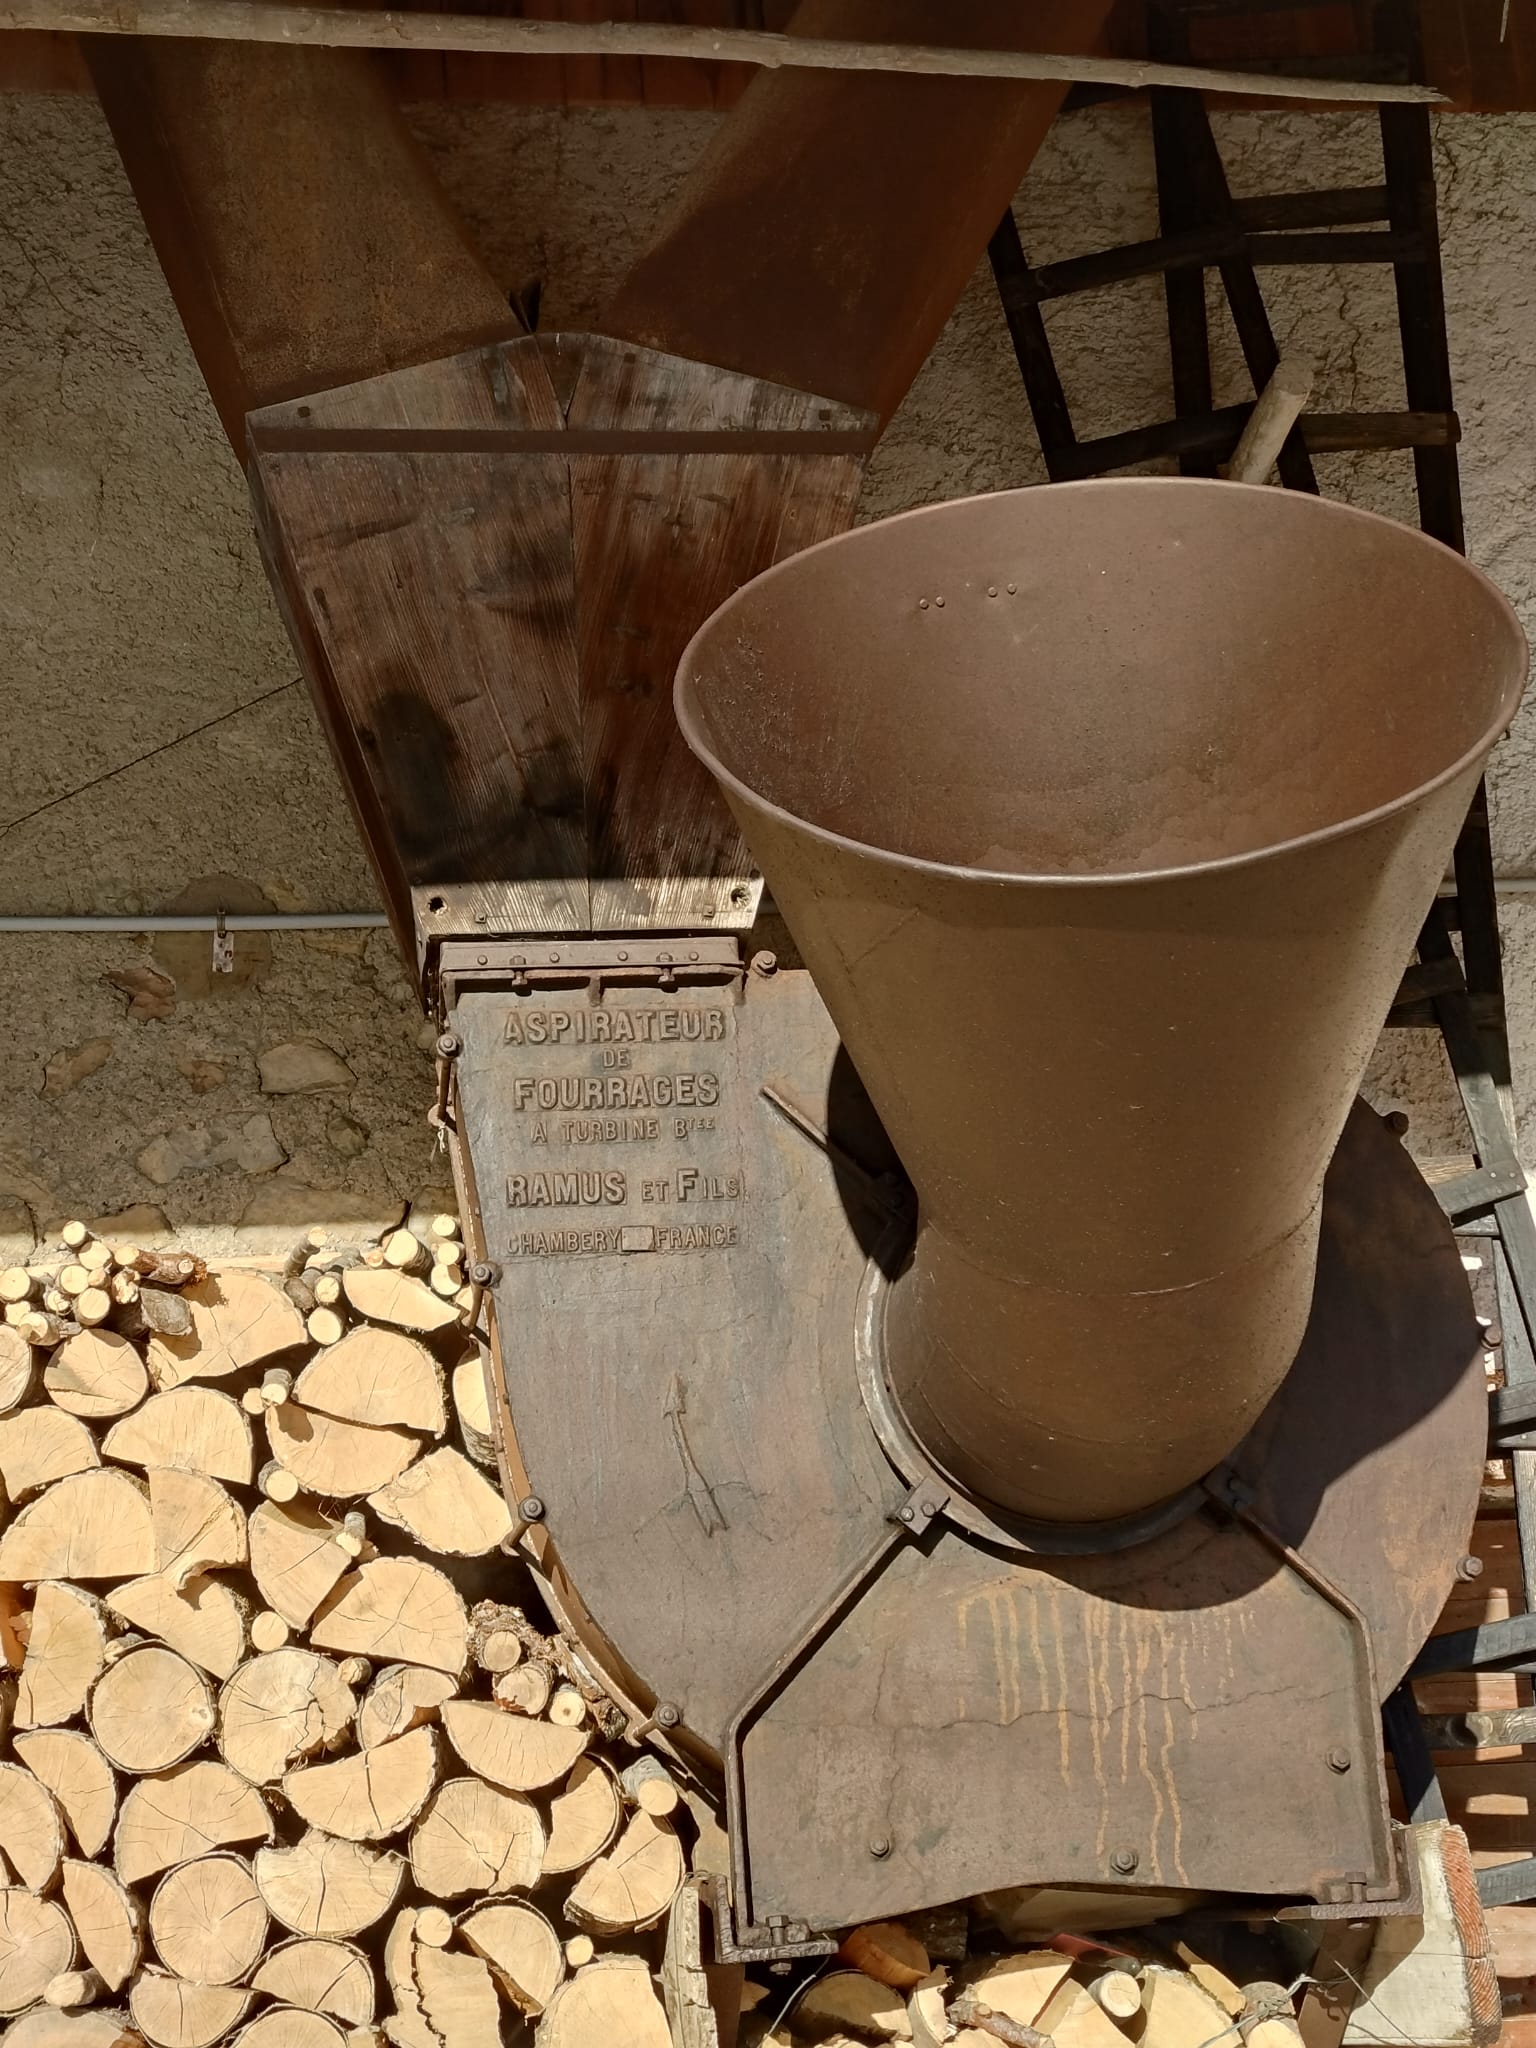
\includegraphics[width=\textwidth]{images/other/pompe_centrifuge.jpg}
        \caption{Old centrifugal pump used to move hay (personal picture)}
        \label{fig:old_centrifugal_pump}
    \end{subfigure}
    \hfill
    \begin{subfigure}[b]{0.61\textwidth}
        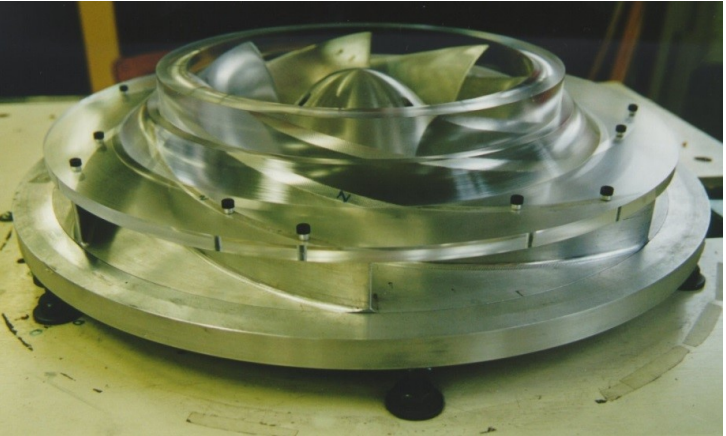
\includegraphics[width=\textwidth]{images/experimentalPump/RESEDA_benchmark_impeller_pic.png}
        \caption{SHF impeller used in the RESEDA benchmark}
        \label{fig:RESEDA_benchmark_impeller}
    \end{subfigure}
    \caption{Centrifugal pumps}
\end{figure}

Different high-fidelity data has been recorded on the diffuser of the pump at the LMFL:
\begin{itemize}[nosep]%, left=0pt]
    \item High-Speed \ac{PIV} data obtained by Dazin et al.~\cite{dazinHighspeedStereoscopicPIV2011a} in 2011;
    \item pressure data obtained by Fan et al.~\cite{fanEffectLeakagePerformanceb} in 2022.
\end{itemize}

Both experimental (traditionally) and numerical (increasingly in recent years) approaches have been used to investigate the rotor-stator interactions to improve performance, develop accurate models and permit real-time monitoring and control.

\paragraph{CFD} To obtain a numerical simulation of the flow in the pump, a \ac{CFD} can be performed.
There are different ways to discretize the space when we do CFD (see \autoref{fig:solidworksMesh}\footnote{\url{https://www.solidworks.com/sw/docs/flow_basis_of_cad_embedded_cfd_whitepaper.pdf}}). The most common are structured meshes, unstructured meshes and body-fitted meshes.
\begin{figure}[H]
    \centering
    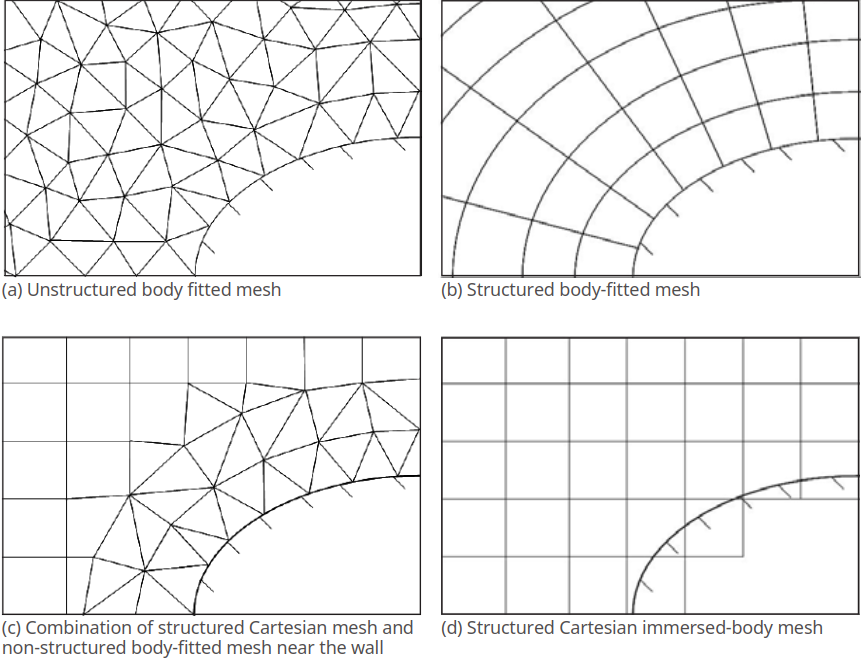
\includegraphics[width=0.8\textwidth]{images/solidworksMesh3.png}
    \caption{Differents strategies for meshing}
    \label{fig:solidworksMesh}
\end{figure}
A structured mesh is a mesh whose connectivity between points can be described in a regular manner, typically using multidimensional arrays (1D, 2D, 3D). In such a mesh, the points are organized in a regular grid, allowing easy navigation through the data.
In contrast, an unstructured mesh is a mesh where cells cannot be described in a regular manner. They are defined by arbitrary geometric shapes where the connectivity of the points does not follow a regular pattern. These meshes are often used to model complex geometries where a regular grid would be unsuitable. %This means that each cell must explicitly specify the points that compose it, in a specific order.

The body-fitted meshes are the most accurate but also the most expensive in terms of computational resources in case the grids update at each time step.

\paragraph{IBM} is a numerical technique that simulates viscous flow with embedded boundaries on grids that do not conform to those boundaries. This allows to keep numerical efficiency on complex geometries and moving boundaries without the need for body-fitted meshes, which can be computationally expensive and difficult to implement.

In 1972 Charles S. Peskin\cite{IBM_base} developped the IBM method. His goal was to reduce the computational time, mainly due to the computation of the mesh refinment based on the \ac{CFL} (see \autoref{eq:CFL}). He added an IBM forcing term on Navier-Stokes equations, only on the simulated artificial heart valve part. He overcame the numerical instabilitys due to the boundary forces by using an iterative method for solving a fixed-point problem for boundary forces.

In 1999 Angot et al. \cite{angotPenalizationMethodTake1999a} discovered that using the penalization IMB, the velocity penalized at the wall was the same as the one from a body-fitted approach if $\mathbf{D}$, a forcing parameter defines in the \autoref{subsec:CFD_governing_equations}, tend to infinity.

IBM are usually less accurate and need more cells element to keep good precision in the near-wall region, but more efficient in terms of computational resources when the geometry is moving. So it's more and more used in CFD \cite{annurev:/content/journals/10.1146/annurev-fluid-120720-022129}. The maths behind the method are detailed in the \autoref{eq:IBM}.


\paragraph{Data Assimilation} \ac{DA} is a technique used to improve the accuracy of numerical models by combining them with observational data\cite{aschDataAssimilationMethods2016}. It is widely used in various fields, including meteorology, oceanography, and engineering. The goal of DA is to obtain a more accurate representation of the state of a system by integrating information from different physical measurements or hight-fidelity sources.


There exist many methods for data assimilation, distributed in three main categories: \textbf{variational}, \textbf{statistical} and \textbf{hybrid} methods (see \autoref{fig:DAmap}).
\begin{itemize}
    \item Variational methods (also called classical methods), such as the 3D-Var and 4D-Var, use optimization techniques to find the best estimate of the state of a system by minimizing the difference between model predictions and observations\cite{rabierVariationalDataAssimilation};
    \item Statistical methods (also called sequential methods), such as the Kalman filter and its \ac{EnKF} variant, update the model state iteratively as new observations become available\cite{aschDataAssimilationMethods2016}. It is working by maximizing a certain \ac{PDF} $\left\langle e^a \right\rangle_k = 0$;
    \item Hybrid methods, which combine both variational and statistical approaches. They are not discussed here, as they were not used in this work and fall outside the scope of our study.
\end{itemize}


\begin{figure}[H]
    \centering
    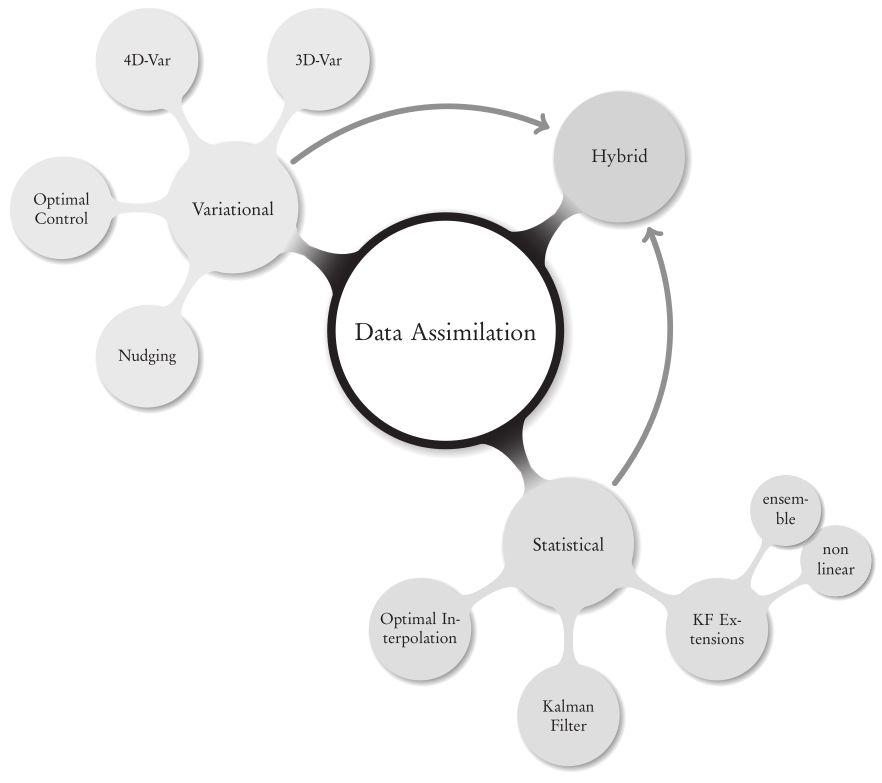
\includegraphics[width=0.7\textwidth]{images/other/DAmap.png}
    \caption{The big picture for DA methods and algorithms\cite{aschDataAssimilationMethods2016}}
    \label{fig:DAmap}
\end{figure}


\paragraph{EnKF} The EnKF, is a statistical Monte Carlo DA method that uses a set of model states (reffered to as ensemble member) to estimate the state of the system. The EnKF is particularly a well-suited tool for assimilating data on nonlinear and high-dimensional systems and has been successfully applied in various fields, including \ac{CFD} simulations, allowing for the correction of model predictions based on observed data.
%The EnKF method is a powerful tool for assimilating data into CFD simulations, allowing 
It mainly consists of two steps:
\begin{itemize}
    \item \textbf{Forecast}: time advancement of the different model states or ensemble members;
    \item \textbf{analysis}: correction of the model prediction by some measured observation describing the same physical phenomenon.
\end{itemize}
The maths behind the EnKF method are detailed in the \autoref{subsec:EnKF}.

\begin{figure}[H]
    \centering
    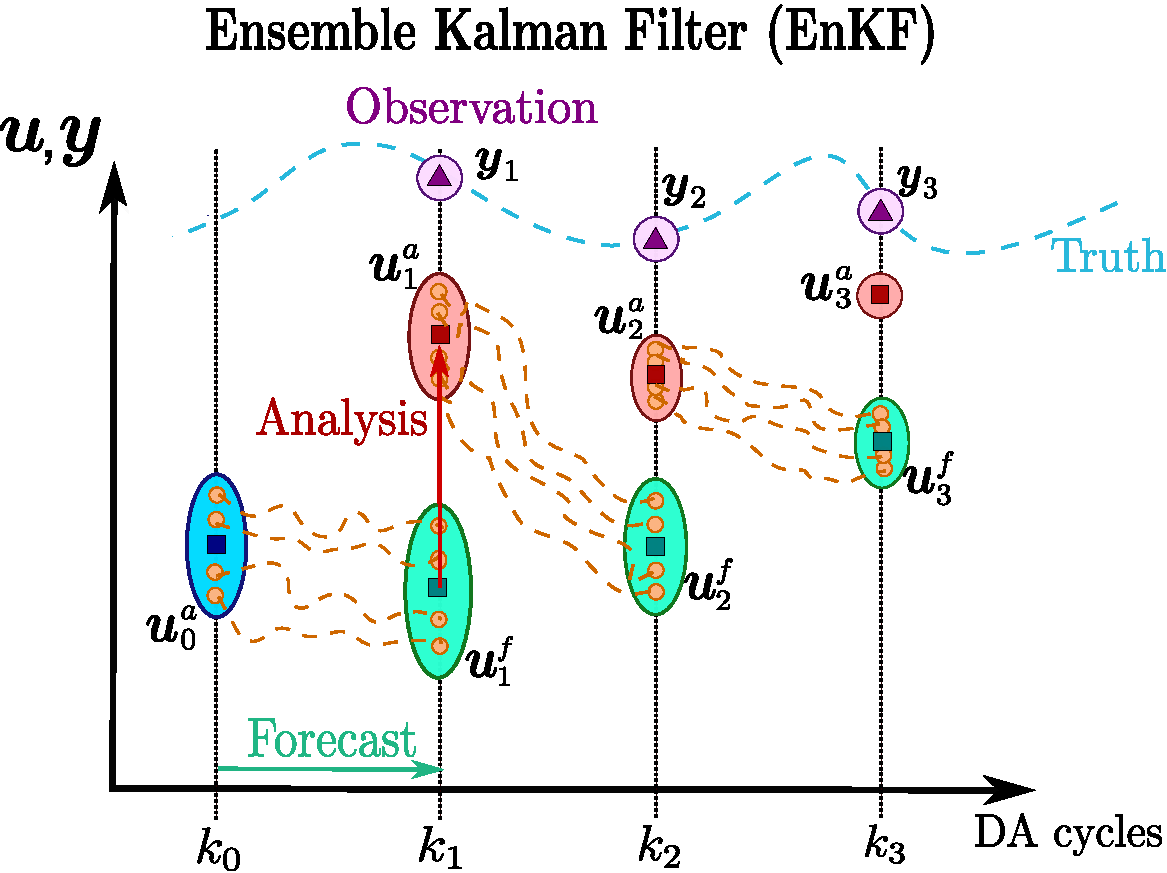
\includegraphics[width=0.60\textwidth]{images/EnKF_algorithm.pdf}
    \caption{Illustration of the EnKF process (100\% confidence in observations)}
    \label{fig:EnKFIllustration}
\end{figure}

EnKF for DA in CFD has been used at \ac{LMFL} for a few years now.
\begin{itemize}
    \item In 2023, Lucas Villanueva, with Miguel M.Valero and Marcello Meldi from LMFL wrote an article\cite{villanuevaAugmentedStateEstimation2023} about the amelioration of the flow around a building preforming EnKF on five CFD parameters, showing a global improvement for both the velocity field and the pressure field;
    \item In 2024, Tom Moussie, with Paolo Errante and Marcello Meldi from LMFL wrote an article\cite{moussieStatisticalInferenceUpstream2024a} successfully optimizing the boudary condition of the academical rectangular 5:1 cylinder benchmarck using EnKF, leading to a significant improvement of the accuracy in the prediction of the turbulent flow;
    \item This year, Miguel M.Valero and Marcello Meldi published an article combining EnKF, \ac{ML} and IBM on a turbulent channel flow \cite{valeroEnhancedStateEstimation2025}. It shows that this combination can gives very good and low cost results;
    \item During my internship, Tom Moussie submitted an article on the determination of the incidence angle of a 2D wing using EnKF, and Miguel also submitted also an article about the optimization of forcing parameters of an IBM around an 2D oscillating cylinder, showing very good results.
\end{itemize}



%An illustration of the EnKF data assimilation process is shown in Figure \ref{fig:EnKFIllustration}.


% Je cherche à transmettre quelle idée ?
% State of art: ce qui a été fait avant, ce qui est fait aujourd'hui, ce qui est fait dans le cadre de mon stage


%(Article in writing process)


This led us to explore the use of the EnKF method to optimize the parameters of the IBM forcing term on a centrifugal pump — a more complex case than the previous ones. It combines the 3D turbulent boundary layer characteristics of the turbulent plane channel flow with the moving body configuration of the oscillating cylinder. Its complex geometry requires around 11 million cells. On top of that, rotor/stator interaction in centrifugal machines is highly unsteady and involves turbulent boundary layers and instabilities, making it particularly challenging to model. Traditional CFD approaches often fail to capture these effects accurately. Our goal here is to improve flow prediction at the diffuser by optimizing the IBM forcing parameters, which should enhance the overall simulation and provide a better understanding of the pump’s behavior.

\newpage

In this context, we aim to apply both of these innovative methodologies to enhance the original CFD predictions on a centrifugal pump test case. The approach leverages PIV measurements at the diffuser, along with pressure tap data from the impeller inlet and the diffuser. To achieve this, the thesis is organized around the following steps:

\begin{enumerate}
    \item Do a state of the art about the centrifugal pumps, CFD methods including IBM and DA including EnKF, detail in this \autoref{sec:stateOfArt};
    \item understand some numerical ingredients as CFD governing equations, the open-source code OpenFoam, the EnKF method, the CONES library and the pump modeling that are explained in the \autoref{subsec:CFD_governing_equations};
    \item pre-process the experimental data to be able to compare them to the numerical model, \autoref{sec:Experimental_data_and_pre-processing};
    \item modify OpenFOAM to obtain first simulation results using IBM, \autoref{sec:IBM_preliminary_results};
    \item modify CONES to adapt it to the pump case and apply the DA to modify the IBM parameters, \autoref{sec:Application_of_the_DA};
    \item analyse the results of the DA on the optimization of the field in the diffuser and the accuracy of the perfomance of the pump, \autoref{sec:Results}.
\end{enumerate}


% Puis amener cas 3 (pompe) pour transitionnre vers la sous-parite suivante

%\label{subsec:Presentation_of_the_data_from_the_centrifugal_pump_test_case}




%The pdf is a paper where can be found the experimental conditions even if the analysis are focussed on another flow rate.

%Détail: R3 = 0.257m; h=0.0400m; Q = 0.236m3/s -> S=0.0646m2

%\title{Fonctionning}  % ????
%\title{Utility}


\hspace{1cm}

\newpage

\section{Numerical ingredients}

\subsection{CFD governing equations}
\label{subsec:CFD_governing_equations}

\paragraph{Navier-Stokes equations} CFD is based on the fundamental equations of fluid mechanics. When the fluid is assumed to be Newtonian, these equations reduce to the nonlinear Navier–Stokes partial differential equations.

These equations express three physical conservation principles, given here in their Eulerian form (i.e., fixed spatial reference frame), which is the standard in CFD because it describes how fluid properties evolve at fixed locations in space, which is ideal for mesh-based numerical simulations.


%\[
%\boldsymbol{\tau}
%= \mu\big(\nabla\mathbf{U}+(\nabla\mathbf{U})^{\!\top}\big)
%-\tfrac{2}{3}\mu\,(\nabla\!\cdot\mathbf{U})\,\mathbf{I},

%\rho\Big(\frac{\partial \mathbf{U}}{\partial t}+(\mathbf{U}\cdot\nabla)\mathbf{U}\Big)
%= -\,\nabla P + \mu\nabla^{2}\mathbf{U}
%+ (\mu+\lambda)\,\nabla(\nabla\!\cdot\mathbf{U}) + \mathbf{f},

%\rho\Big(\frac{\partial \mathbf{U}}{\partial t}+(\mathbf{U}\cdot\nabla)\mathbf{U}\Big)
%= -\,\nabla P + \mu\nabla^{2}\mathbf{U} + \mathbf{f}.
%\]


\begin{itemize}
    \item \textbf{Mass conservation (Continuity equation):}
    \begin{equation}
        \frac{\partial \rho}{\partial t} + \text{div}(\rho \mathbf{U}) = 0   %         \frac{\partial \rho}{\partial t} + \nabla \cdot (\rho \mathbf{U}) = 0
        \label{eq:mass_conservation}
    \end{equation}

    with $\rho$ the density and $\mathbf{U}$ the velocity.

    \item \textbf{Momentum conservation (second Newton Law):}     % (Navier–Stokes equation)
    \begin{equation}
        \rho\Big(\frac{\partial \mathbf{U}}{\partial t}+(\mathbf{U}\cdot\nabla)\mathbf{U}\Big) = -\,\nabla P + \nabla\!\cdot\boldsymbol{\tau} + \mathbf{f}
    \end{equation}
    where $P$ is the pressure, \( \boldsymbol{\tau} \) is the viscous stress tensor and \( \mathbf{f} \) includes body forces (e.g., gravity, source terms).

    \item \textbf{Energy conservation (First law of thermodynamics):}
    \begin{equation}
        \frac{\partial (\rho E)}{\partial t} + \nabla \cdot (\mathbf{U} (\rho E + P)) = \nabla \cdot (k \nabla T) + \Phi
    \end{equation}
    where \( k \) is the thermal conductivity, \( T \) the temperature, and \( \Phi \) the viscous dissipation and $e$ the potential energy.
    $E = e + \frac{1}{2} \boldsymbol{U}^2$ is the total energy per unit mass, with:

    \begin{itemize}
        \item $e$: internal energy per unit mass (also called specific internal energy)
        \item $\frac{1}{2} \boldsymbol{U}^2$: kinetic energy per unit mass (specific kinetic energy)
    \end{itemize}

    For an ideal gas, the internal energy is generally given by $e = c_v T$, where:
    \begin{itemize}
        \item $c_v$ is the specific heat capacity at constant volume
        \item $T$ is the temperature
    \end{itemize}
\end{itemize}

Two main indicators of the main behaviour of the flow are the \ac{Ma} and the \ac{Re}.

The $Ma$, is defined by the velocity of the flow divided by the speed of the sound (relative to the flow). In CFD, flow is usually considered as incompressible for Mach lower than 0.3.
In our case, in atmospheric conditions,

\begin{equation}
    Ma = \cfrac{R_2 \Omega}{c} < 0.095 \phantom{-} \textrm{\textbf{(incompressible)}}
\end{equation}

With $R_2 = 0.2575m$ the external radius of the impeller, $\Omega = 2\pi \times 1200/60 = 125.7 rad/s$ the angular velocity of the impeller and $c = 343 m/s$ the speed of sound in air at 15°C.

As we consider that we are in \textbf{incompressible} flow conditions (because we are at low Ma), \autoref{eq:mass_conservation} becomes
\begin{equation}
    \nabla \cdot \mathbf{U} = 0
\end{equation}
And the pressure and velocity are solved iteratively, contrary to compressible flows.

The dimensionless $Re$ measures the ratio between inertial and viscous forces. It indicates if the flow is turbulent, laminar or both, it caratcterizes the flow regime. 
Let's compute the $Re$ around where the velocity should be the highest.

\begin{equation}
    Re = \frac{UL}{\nu}
\end{equation}

$U$ is the velocity of the fluid, $L$ is the characteristic length and $\nu$ the kinematic viscosity of the fluid.

\begin{equation}
    Re_{r_{tip}}=\cfrac{R_2^2 \Omega}{\nu} = 5.53\times10^5
\end{equation}




\begin{comment}
- Conservation de la quantité de mouvement, équation de bilan de la quantité de mouvement: 

- Conservation de l'éngergie: 
...
\textbf{Conservation de la quantite de mouvement (équation de NavierStokes)}:
\[
    \rho \left( \frac{\partial \mathbf{u}}{\partial t} + (\mathbf{u} \cdot \nabla)\mathbf{u} \right) = -\nabla p + \mu \nabla^2 \mathbf{u} + \mathbf{f}
\]

\textbf{Conservation de l energie}:
\[
    \rho \left( \frac{\partial e}{\partial t} + \mathbf{u} \cdot \nabla e \right) = -p \nabla \cdot \mathbf{u} + \Phi
\]
équations de Navier-Stokes incompressibles, isothermes, en coordonnées cartésiennes:

\begin{itemize}
    \item \textbf{Conservation de la masse (équation de continuité)}:
    \[
        \frac{\partial u}{\partial x} + \frac{\partial v}{\partial y} + \frac{\partial w}{\partial z} = 0
    \]

    \item \textbf{Conservation de la quantité de mouvement (x, y, z)}:
    \[
        \rho \left( \frac{\partial u}{\partial t} + u\frac{\partial u}{\partial x} + v\frac{\partial u}{\partial y} + w\frac{\partial u}{\partial z} \right) = -\frac{\partial p}{\partial x} + \mu \left( \frac{\partial^2 u}{\partial x^2} + \frac{\partial^2 u}{\partial y^2} + \frac{\partial^2 u}{\partial z^2} \right)
    \]
    \[
        \rho \left( \frac{\partial v}{\partial t} + u\frac{\partial v}{\partial x} + v\frac{\partial v}{\partial y} + w\frac{\partial v}{\partial z} \right) = -\frac{\partial p}{\partial y} + \mu \left( \frac{\partial^2 v}{\partial x^2} + \frac{\partial^2 v}{\partial y^2} + \frac{\partial^2 v}{\partial z^2} \right)
    \]
    \[
        \rho \left( \frac{\partial w}{\partial t} + u\frac{\partial w}{\partial x} + v\frac{\partial w}{\partial y} + w\frac{\partial w}{\partial z} \right) = -\frac{\partial p}{\partial z} + \mu \left( \frac{\partial^2 w}{\partial x^2} + \frac{\partial^2 w}{\partial y^2} + \frac{\partial^2 w}{\partial z^2} \right)
    \]
\end{itemize}
\end{comment}


%\paragraph{Turbulence modelling}  This equations permit runnig all the scales in case of turbulent flows, i.e. a \ac{DNS}, that would be too costly in our case.
%The Kolmogorove scale, define by the spatial scale from which viscosity allows the kinetic energy of a flow to be dissipated, is very small. In fluid mechanics, turbulent flows consist of several scales which are responsible for different phenomena. As illustrated in the following \autoref{fig:Modelisation_of_turbulence}\footnote{\url{https://www.cfdsupport.com/openfoam-training-by-cfd-support/node346/}} and \autoref{fig:Turbulence3}\footnote{\url{https://help.altair.com/hwcfdsolvers/acusolve/topics/acusolve/training_manual/turbulence_modeling_r.htm}}, large scales are responsible dor the production of turbulence and energy, whiwh is shifted through the inertial range toward the Kolmogorov scale, responsible for the dissipation phenomena.
%There are two major ways to model the turbulence.
%The first one is by using \ac{LES}, that simulates only the small scale eddy usually in the near-wall region.
%The second one is the \ac{RANS} that model every scall of eddy. The result is a stady-state and it less precise but fastly computed than LES.
%The \autoref{fig:Turbulence2}\footnote{\url{https://blog.diphyx.com/comprehensive-guide-review-to-choosing-the-right-cfd-software-in-2023-features-performance-and-7ebc0623bfa6}} illustrates well a visualization of the fiels of the three type of CFD models.


In turbulent flows, a wide range of spatial and temporal scales coexist. Solving the Navier–Stokes equations without any turbulence model (i.e., via \textbf{Direct Numerical Simulation (DNS)}) would theoretically capture all these scales. However, DNS is computationally unaffordable in most practical cases, as it requires resolving down to the smallest dissipative scales, known as Kolmogorov scales.

These Kolmogorov scales define the smallest spatial structures in the flow where kinetic energy is dissipated by viscosity. As shown schematically in Figure~\ref{fig:Turbulence3}\footnote{\url{https://help.altair.com/hwcfdsolvers/acusolve/topics/acusolve/training_manual/turbulence_modeling_r.htm}}, turbulence consists of large energy-containing eddies, which transfer their energy through a cascade in the inertial range, down to the smallest dissipative structures.

To reduce computational cost, turbulence modelling is employed. Two main approaches exist:
\begin{itemize}
    \item \textbf{Large Eddy Simulation (LES)}: it resolves the large, energy-carrying structures and models only the small-scale turbulence. LES is more accurate than RANS but more computationally expensive, particularly near walls (see Figure~\ref{fig:Turbulence1})\footnote{\url{https://www.cfdsupport.com/openfoam-training-by-cfd-support/node346/}}.
    \item \textbf{Reynolds-Averaged Navier–Stokes (RANS)}: it models the entire turbulence spectrum through statistical averaging and closure models. It is less accurate but significantly cheaper, often used in steady-state simulations.
\end{itemize}

Note that DNS and LES do not rely on turbulence models in the traditional sense like RANS does; instead, they resolve directly or partially turbulence dynamics. Also, caution must be taken when interpreting visual comparisons of DNS, LES, and RANS fields (see Figure~\ref{fig:Turbulence2})\footnote{\url{https://blog.diphyx.com/comprehensive-guide-review-to-choosing-the-right-cfd-software-in-2023-features-performance-and-7ebc0623bfa6}}, as the underlying assumptions and modelling strategies differ.



\begin{figure}[H]

\end{figure}

\begin{figure}[H]
    \begin{subfigure}{0.48\textwidth}
    \centering
        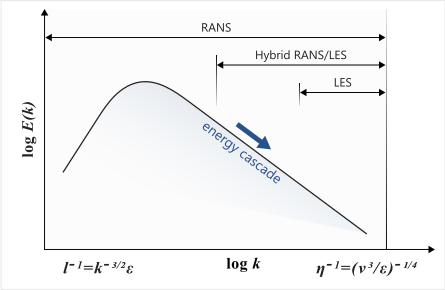
\includegraphics[width=1\textwidth]{images/turbCascade.png}
        \caption{Turbulence model on the energy cascade}
        \label{fig:Turbulence3}
    \end{subfigure}
    \begin{subfigure}{0.41\textwidth}
    \centering
        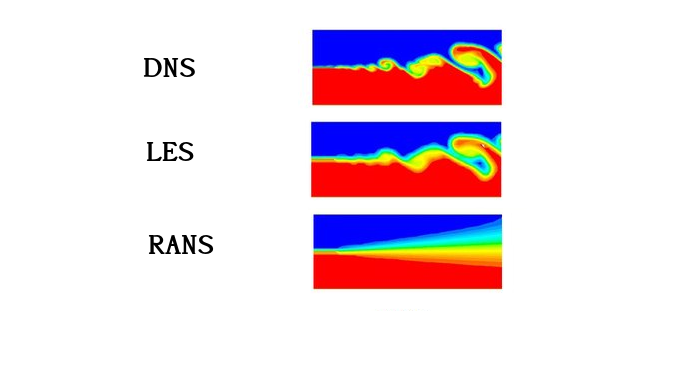
\includegraphics[width=1\textwidth]{images/DNSLESRANS.png}
        \caption{Illustration of different CFD models}
        \label{fig:Turbulence2}
    \end{subfigure}
    \hfill
    \centering
    \begin{subfigure}{0.75\textwidth}
        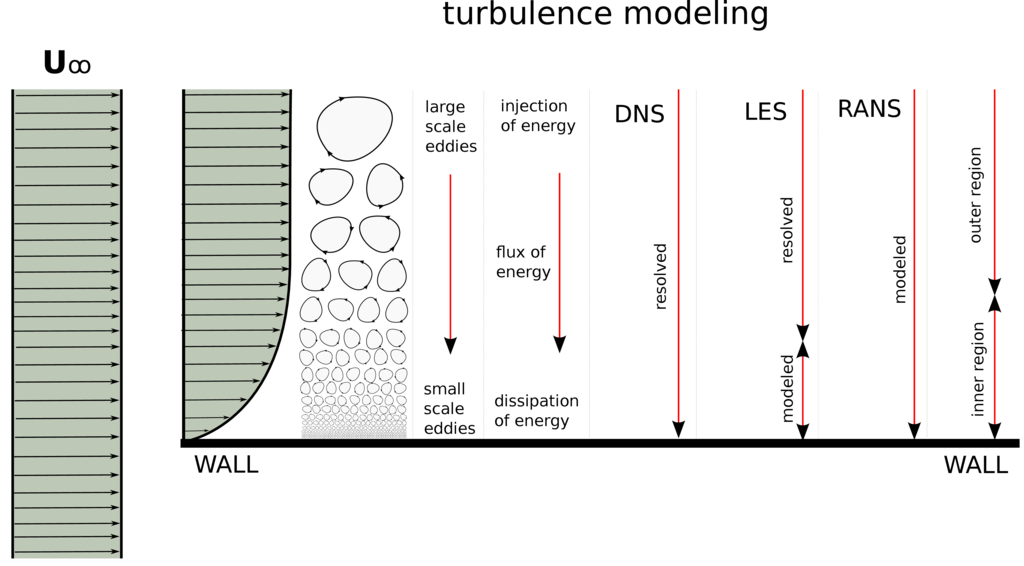
\includegraphics[width=1\textwidth]{images/sketch-turbulent-flow-modeling-DNS-LES-RAS.png}
        \caption{Near wall modelisation of turbulence}
        \label{fig:Turbulence1}
    \end{subfigure}
    \caption{Turbulence models}
    \label{fig:Modelisation_of_turbulence2}
\end{figure}

In our study, we are going to have a look on the \ac{U-RANS} method using the same principle as the RANS method but it's unsteady, allowing to make turn physically the pump in our case.

More precisely, in our RANS and U-RANS simulation, we are going to use a $k-\omega$ \ac{SST} turbulence model. It is a two-equation eddy-viscosity model: it combines the $K-\epsilon$ and the $K-\omega$ turbulence approximations plus a blending region between both.

$K-\omega$ is known to be a good model in the near-wall region but a bad prediction in bulk flow.
$K-\epsilon$ makes a good numerical prediction in the bulk flow field but is less accurate near solid surfaces.

\begin{figure}[H]
    \centering
    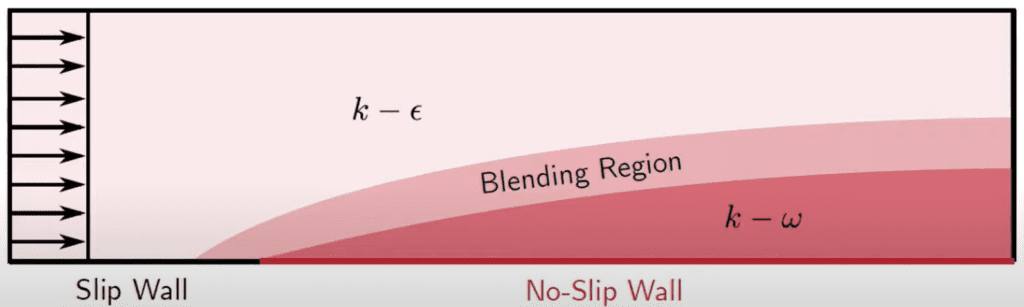
\includegraphics[width=0.65\textwidth]{images/k-omega-sst.png}
    \caption{$k-\omega SST$ model}
    \label{fig:kOmega_SST}
\end{figure}

$k-\omega SST$ model is defined as follows\footnote{\url{https://www.cfd-online.com/Wiki/SST_k-omega_model}}\cite{doi:10.2514/6.1993-2906}\cite{doi:10.2514/3.12149}:


- Norm of the strain tensor
\begin{equation}
    % Définition de S (norme du tenseur de déformation)
    S = \sqrt{2 S_{ij} S_{ij}}, \quad \text{avec } S_{ij} = \frac{1}{2} \left( \frac{\partial U_i}{\partial x_j} + \frac{\partial U_j}{\partial x_i} \right)
\end{equation}

- Kinematic Eddy Viscosity:
\begin{equation}
    \nu _T  = {\frac{a_1 k}{\mbox{max}(a_1 \omega, S F_2)}}
\end{equation}

- Turbulent kinetic energy production term
\begin{equation}
    % Définition de P_k (terme de production de l'énergie cinétique turbulente)
    P_k = \tau_{ij} \frac{\partial U_i}{\partial x_j}
\end{equation}

- Turbulence Kinetic Energy:
\begin{equation}
    \frac{\partial k}{\partial t} + U_j \frac{\partial k}{\partial x_j} = P_k - \beta^* k\omega + \frac{\partial}{\partial x_j} \left[ \left( \nu + \sigma_k \nu_T \right) \frac{\partial k}{\partial x_j} \right]
\end{equation}


- Specific Dissipation Rate:
\begin{equation}
    \frac{\partial \omega}{\partial t} + U_j \frac{\partial \omega}{\partial x_j} = \alpha S^2 - \beta \omega^2 + \frac{\partial}{\partial x_j} \left[ \left( \nu + \sigma_{\omega} \nu_T \right) \frac{\partial \omega}{\partial x_j} \right] + 2(1 - F_1)\sigma_{\omega 2} \frac{1}{\omega} \frac{\partial k}{\partial x_i} \frac{\partial \omega}{\partial x_i}
\end{equation}


- Closure Coefficients and Auxiliary Relations:
\begin{equation}
    F_2 = \tanh \left[ \left[ \max \left( \frac{2\sqrt{k}}{\beta^* \omega y}, \frac{500 \nu}{y^2 \omega} \right) \right]^2 \right]
\end{equation}

\begin{equation}
    P_k = \min \left( \tau_{ij} \frac{\partial U_i}{\partial x_j}, 10\beta^* k \omega \right)
\end{equation}

$F_1$ controls the blending between the $k-\epsilon$ and $k-\omega$ models. $F_1$ corresponds to the $k_\epsilon$ model and $F_1 = 1$ corresponds to the $k_\omega$ model.

\begin{equation}
    F_1 = \tanh \left\{ \left\{ \min \left[ \max \left( \frac{\sqrt{k}}{\beta^* \omega y}, \frac{500 \nu}{y^2 \omega} \right), \frac{4 \sigma_{\omega 2} k}{CD_{k\omega} y^2} \right] \right\}^4 \right\}
\end{equation}

\begin{equation}
    CD_{k\omega} = \max \left( 2\rho \sigma_{\omega 2} \frac{1}{\omega} \frac{\partial k}{\partial x_i} \frac{\partial \omega}{\partial x_i}, 10^{-10} \right)
\end{equation}

$\phi = \phi_1 F_1 + \phi_2 (1 - F_1)$

$\alpha_1 = \frac{5}{9}, \quad \alpha_2 = 0.44$

$\beta_1 = \frac{3}{40}, \quad \beta_2 = 0.0828$

$\beta^* = \frac{9}{100}$

$\sigma_{k1}  = 0.85,  \sigma_{k2}  = 1$

$\sigma_{\omega 1}  = 0.5,  \sigma_{\omega 2}  = 0.856$


On the $\omega$ region, we can define a near-wall model where the mesh is too coarsed to capture the inner sublayer (see \autoref{fig:NearWallModelling})\footnote{\url{https://2021.help.altair.com/2021/hwsolvers/acusolve/topics/acusolve/training_manual/near_wall_modeling_r.htm}}.

We can define the nomalized wall ditance as:
\begin{equation}
    y^+ = \frac{\rho u_{tau} y}{\mu}
\end{equation}
where $y$ is the distance from the wall and $\mu$ the fluid dynamic viscosity.
This will allows us to know where to use a near-wall model.

\begin{figure}[H]
    \centering
    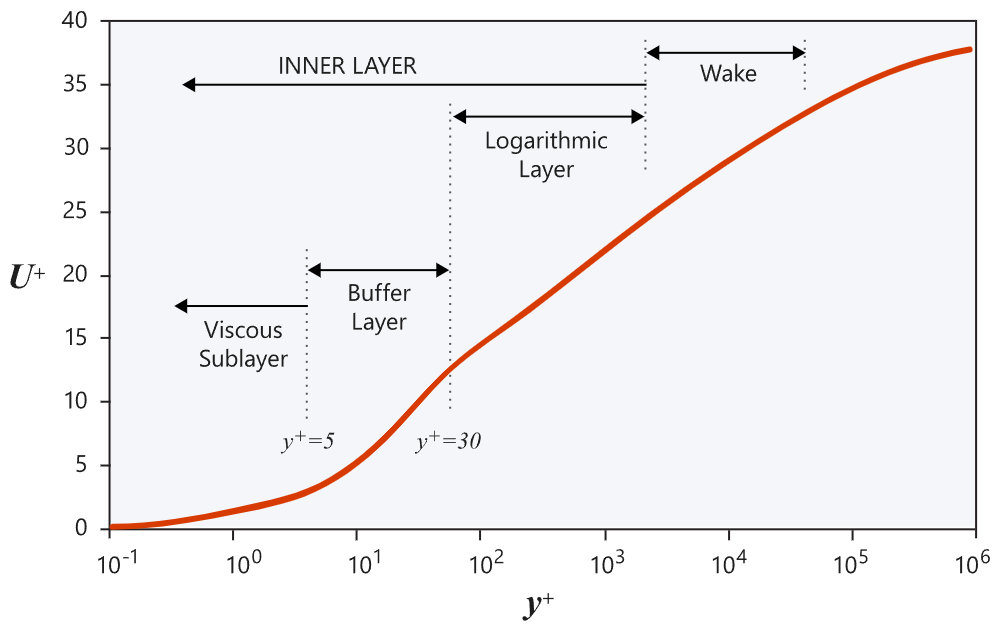
\includegraphics[width=0.7\textwidth]{images/NearWallModelling.png}
    \caption{Near wall model}
    \label{fig:NearWallModelling}
\end{figure}


\paragraph{MRF method}
To simulate the rotation of the impeller in a steady-state RANS simulation, we use the \ac{MRF} method. The MRF strategy consists in solving the Navier-Stokes equations in a rotating reference frame in the rotating region, while keeping the rest of the domain in a stationary (inertial) frame. The mesh and geometry remain static; only the reference frame changes.

The governing equations in the rotating frame (relative velocity) are derived from the Navier-Stokes equations in the inertial frame by applying a transformation that accounts for the rotating frame accelerations.

For an incompressible flow, the Navier-Stokes equations in the rotating frame with relative velocity $\vec{u}_R$ are:

\begin{equation}
\begin{cases}
\frac{\partial \vec{u}_R}{\partial t} + \nabla \cdot (\vec{u}_R \otimes \vec{u}_R) + 2 \vec{\Omega} \times \vec{u}_R + \vec{\Omega} \times (\vec{\Omega} \times \vec{r}) = - \nabla \left( \frac{p}{\rho} \right) + \nu \nabla^2 \vec{u}_R \\
\nabla \cdot \vec{u}_R = 0
\end{cases}
\end{equation}

Where:

- $\vec{u}_R$ is the velocity in the rotating frame;

- $\vec{\Omega}$ is the angular velocity vector;

- $\vec{r}$ is the position vector;

- $\rho$ is the fluid density;

- $\nu$ is the kinematic viscosity.

The additional terms $2 \vec{\Omega} \times \vec{u}_R$ (Coriolis force) and $\vec{\Omega} \times (\vec{\Omega} \times \vec{r})$ (centrifugal force) appear due to the non-inertial frame transformation.

\begin{figure}[H]
    \centering
    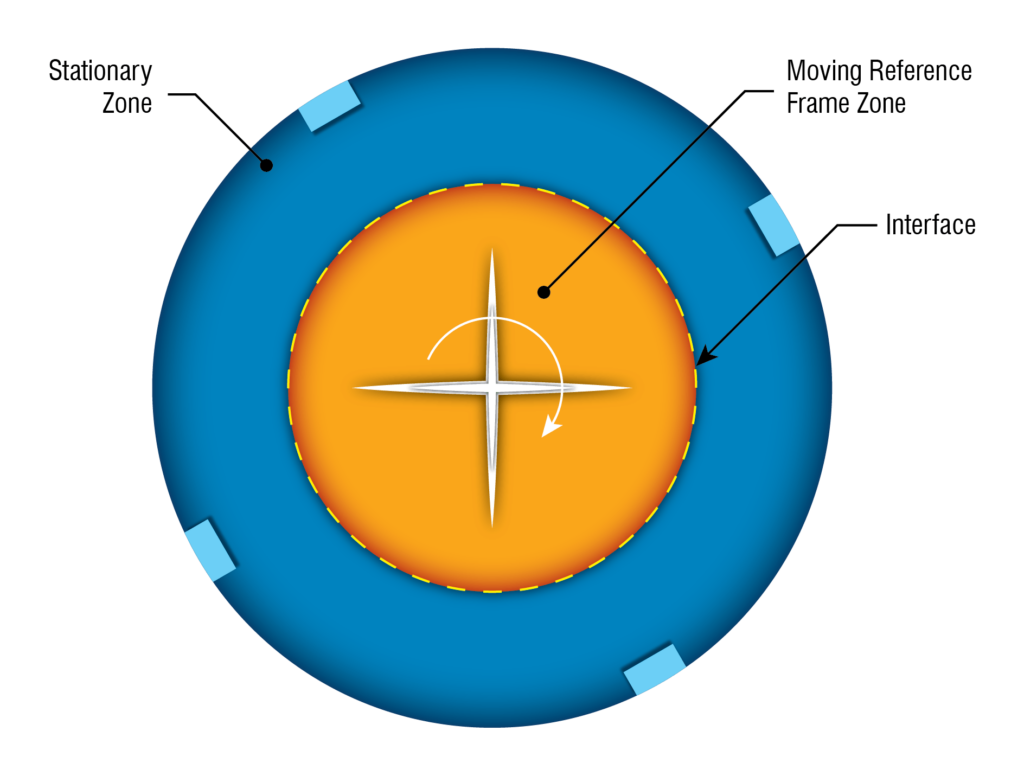
\includegraphics[width=0.62\textwidth]{images/MRF.png}
    \caption{MRF strategy: the rotating region is solved in a non-inertial frame}
    \label{fig:MRF}
\end{figure}




%The principle is to add relative frame term in a moving part while the other part stays fixe. Neither the mesh nor the body is moving.
%The mathematical method is just to resolve the eqations in the stationary zone on one side. On the other side, equations are resolved in the relative frame, then the relativ motion is added. In our case, the relative motion is a constant rotation speed

%Assuming the rotating speed is given in revolutions per minute (rpm), we can convert it to radians per second:
%\begin{equation}
%    \omega = \frac{1200 \text{ rpm} \cdot 2\pi \text{ rad}}{60 \text{ s}} = 125.66 \text{ rps}.
%\end{equation}
%So $\Omega = (0;0;125.66) rad.s^{-1}$ and $U_{abs} = U_{rel} + \Omega \times R$



\paragraph{U-RANS} In the \ac{U-RANS} case, the impeller is physically moving. %Also, very large eddy are simulated.

To do so, the \ac{CFL} or the courant number has to be computed. 

\begin{equation}
    \label{eq:CFL}
    CFL = \frac{\Delta_t}{\Delta_x} \times \mathbf{U}
\end{equation}

Typically set to a maximum of 1 for stability. 

The CFL number can be interpreted as the fraction of the cell size that a disturbance (or wave) travels during a single time step. In this case, it corresponds to the ratio between the distance covered at the impeller tip in one time step and the space between two cells in the azimuthal direction.
%A way to visualize the CFL is to think of it as the fraction of the distance a wave travels in one time step relative to the distance between two cells in the azimuthal direction at the tip of the impeller.
The CFL is computed locally at each mesh element. Let's compute the $\Delta_t$ at the tip of the impeller, where the velocity is the highest and $\Delta_x$ the lowest.

- In our model, $\Delta_{x}$ is the distance between two cells in the azimuthal direction at the tip of the impeller, which is given as 1.5 mm or 0.0015 m.

- $\|U_{\infty}\|$ is the magnitude of the maximal velocity usually "at infinity distance" from the body, which in our case can be approximated by the tangential velocity at the tip of the impeller.

\begin{equation}
    \|U_{\infty}\| = \Omega \cdot r_{tip}
\end{equation}

where:

- $\omega$ is the angular velocity in radians per second,

- $r_{tip}$ is the radius at the tip of the impeller.

Assuming the radius at the tip of the impeller is $r = 0.2566 \text{ m}$, we can compute the tangential velocity:

\begin{equation}
    \|U_{\infty}\| = 125.66 \text{ rps} \cdot 0.2566 \text{ m} =  \text{32.24 m/s}
\end{equation}

Assuming the distance between two cells in the azimuthal direction at the tip of the impeller is $\Delta_{x} = 0.0015 \text{ m}$ (which is 1.5 mm), we can now compute the time step $\Delta_{t}$:

\begin{equation}
    \Delta_{t} = \frac{0.5 \cdot 0.0015 \text{ m}}{32.24 \text{ m/s}} = 2.3 \times 10^{-5} \text{ s} % \approx 2.3 \mu s.
\end{equation}





 %(voir https://fr.wikipedia.org/wiki/%C3%89quations_de_Navier-Stokes)
% Mentionner que les solutions numériques ne sont pas démontrés?//







\paragraph{IBM equations}

As seen in the \autoref{sec:stateOfArt}, different techniques exist to penalise the immersed part. In our case, we are going to use a classical penalisation method proposed by Angot et al.\cite{angotPenalizationMethodTake1999a} which enters the family of continuous forcing approach. Instead of using body-fitted mesh, we are going to consider porous medium and add a forcing term on the Navier-Stokes equations (\autoref{eq:IBMBody}) to simulate the effect of the immersed boundary on the fluid flow. This term is added only on the penalization part $\Omega_b U \Sigma_b$ (see \autoref{fig:IBM_Mesh}).

\begin{figure}[H]
    \centering
    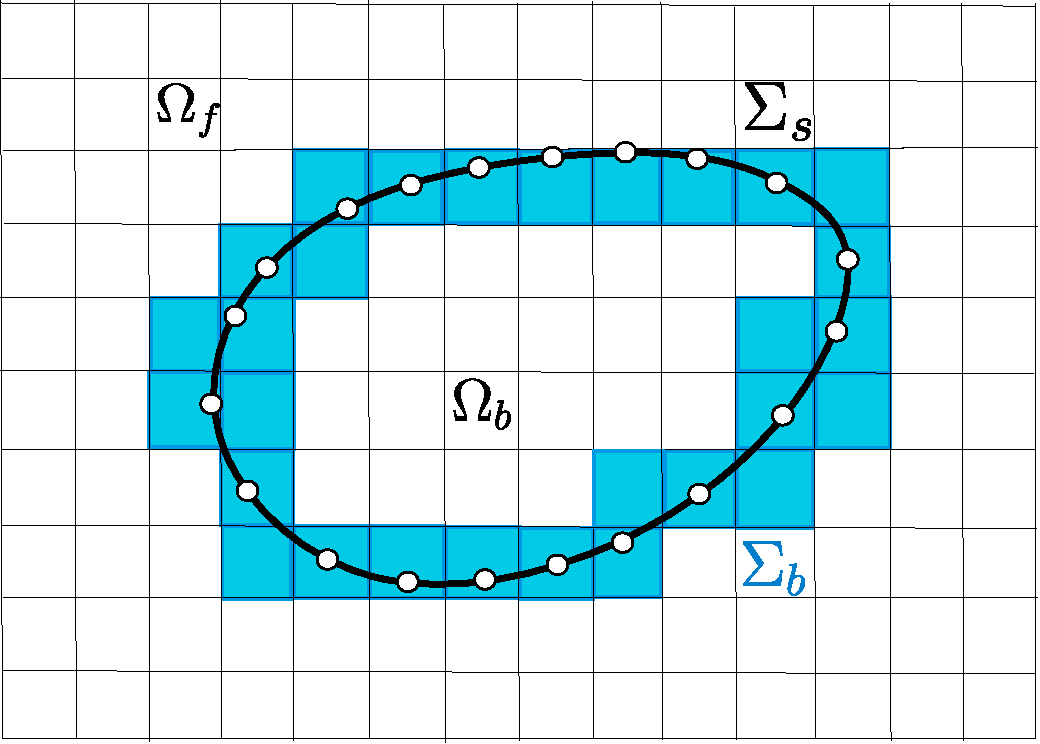
\includegraphics[width=0.45\textwidth]{images/IBM_Mesh.pdf}
    \caption{IBM regions}
    \label{fig:IBM_Mesh}
\end{figure}

The Darcy's law is used in the body interface region $\Sigma_b$ and the solid region $\Omega_b$. To do so, a spatial dependent tensor $\boldsymbol{D}(\boldsymbol{x})$ must be defined. The resulting penalty term is modelled as follows:

\begin{equation}
     \boldsymbol{f}_P = \left\{
        \begin{array}{ll}
        \boldsymbol{0} & \textrm{if } \boldsymbol{x} \in \Omega_f \\
        -\nu \, \boldsymbol{D} \left(\boldsymbol{u} - \boldsymbol{u_{ib}} \right) & \textrm{if } \boldsymbol{x} \in (\Sigma_b \cup \Omega_b)
        \end{array} \right.
    \label{eqn:forcePenDarcy}
\end{equation}

$\boldsymbol{u_{ib}}(\boldsymbol{x}, t)$ is a target velocity representing the immersed body's physical behaviour. In our case, $\boldsymbol{u_{ib}} = \Omega \times \boldsymbol{R}$. The components $D_{ij}$ of the tensor $\boldsymbol{D}$ are usually controlled to obtain the best compromise between the accuracy and stability of the numerical solver.
To converge to the correct result, $\mathbf{D}$ should tend to the infinite. But this lead to numerical instabilities. %$D \rightarrow \infty$, problèmes
%\cite{Verzicco2022_arfm}. The choice performed is crucial in the proximity of the grid transition between the fluid $\Omega_f$ and the interface $\Sigma_b$ regions.

We can also write \autoref{eqn:forcePenDarcy}, once inculding in Naviers-Stokes equations, as:

\begin{equation}
    \label{eq:IBM}
    (\boldsymbol{u} \cdot \boldsymbol{\nabla})\, \boldsymbol{u} = 
    -\frac{1}{\rho} \nabla p + \nu \nabla^2 \boldsymbol{u} 
    \underbrace{- \xi \nu \boldsymbol{D} \left( \boldsymbol{u} - \boldsymbol{u}_{ib} \right)}_{\boldsymbol{f}_P}
\end{equation}
%\begin{equation*}
%    \boldsymbol{\nabla} \cdot (\boldsymbol{u}\boldsymbol{u}) = -\nabla p + \nu \nabla^2 \boldsymbol{u}  \overbrace{-\frac{\xi}{\eta} \left(\boldsymbol{u} - \boldsymbol{u_{ib}} \right)}^{\boldsymbol{f}_P}
%\end{equation*}

\begin{equation}
    \label{eq:IBMBody}
    \xi = \left\{
   \begin{array}{ll}
   0 & \textrm{if } \boldsymbol{x} \in \Omega_f \\
   1 & \textrm{if } \boldsymbol{x} \in (\Sigma_b \cup \Omega_b)
   \end{array} \right.
\end{equation}

%Reprendre ma présentation (dimensiosn de p)

Here, we are dividing both sides of the equations by $\rho$ for simplification which can be considered uniform as we assume incompressible conditions. So $p = \frac{P}{\rho}$, then $[p] = M \cdot L^{-1} \cdot T^{-2}$ and $[\boldsymbol{u}] = L \cdot T^{-1}$

%\begin{equation}
%    \label{eq:IBMBody}
%    \xi = \left\{
%    \begin{array}{ll}
%        0 & \textrm{if } \boldsymbol{x} \in \Omega_f \\
%        1 & \textrm{if } \boldsymbol{x} \in (\Sigma_b \cup \Omega_b)
%    \end{array} \right.
%\end{equation}

As we use a RANS turbulence model, in addition to the velocity, we need to penalize the $k$ and $\omega$ coefficients.




Finnaly, the forcing terms are defined as follows\footnote{\url{https://www.simscale.com/forum/t/defining-turbulent-boundary-conditions/80895}, \url{https://www.openfoam.com/documentation/guides/latest/doc/guide-bcs-wall-turbulence-omegaWallFunction.html}},

\begin{align}
    \label{eq:IB}
    \boldsymbol{f}_{P_u} &= \xi \nu \boldsymbol{D} \left( \boldsymbol{u} - \boldsymbol{u}_{\text{ib}} \right) \\
    \boldsymbol{f}_{P_\mathcal{K}} &= \xi \nu D_{\eta} \left( \mathcal{K} - \mathcal{K}_{\text{ib}} \right) \\
    \boldsymbol{f}_{P_\omega} &= \xi \nu D_{\omega} \left( \omega - \omega_{\text{ib}} \right)
\end{align}



The problem of this method is that $\mathbf{D}, D_{\eta}$ and $D_{\omega}$ need to be tuned to obtain the best results. For that, we use the EnKF method to optimize these constants.




%The maths behind the EnKF method is detailed in the \autoref{subsec:CFD_governing_equations}. 


\subsection{The open-source code OpenFOAM}


Simulations are performed using the C++ framework OpenFOAM, used to discretize the equations previously presented. OpenFOAM is an finite-volume, open-source code which provides many tools, referred to as executables. %\citep[see][]{greenshields2021}. These executable files can be divided into three separate categories:

OpenFOAM provides a wide range of tools for solving the Navier-Stokes equations, including solvers, meshing tools, and post-processing tools. It is widely used in the CFD community and has a large user base. It has been developped since 2004 and is today composed of more than a million lines.

\begin{itemize}
    \item[$-$] \textbf{Pre-processing}, including meshing and decomposing tools;
    \item[$-$] \textbf{Solving}, including in-built and custom solvers. Each solver is built to answer a specific CFD problem;
    \item[$-$] \textbf{Post-processing}, including many tools and libraries to compute post-processing operations. OpenFOAM fields can be visualized with \texttt{ParaView}, an open-source visualization application.
\end{itemize}

OpenFOAM is not provided with a graphical interface, which is why a simulation is built by writing ``dictionaries'', in which is stored the necessary information for the simulation (mesh, turbulence model, maximum number of characteristic times, $\dots$). See tree structure Annex~\ref{annex:OpenFoamArbo}.

%// Ou si plus lisible: //

%\begin{figure}[H]
%    \centering
%    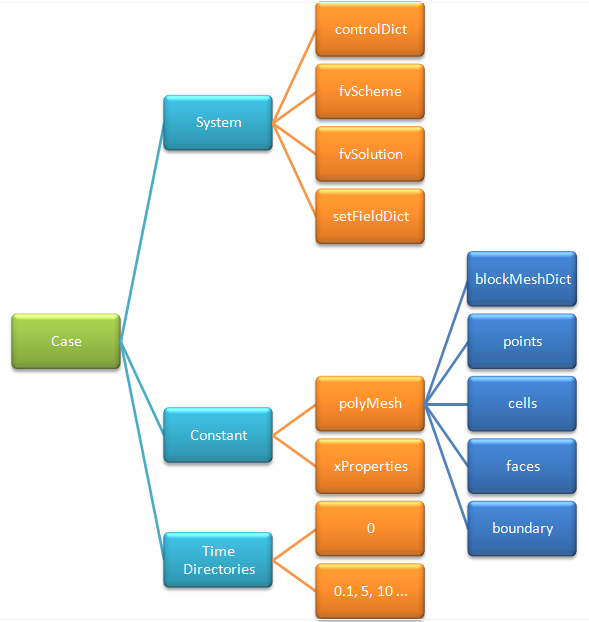
\includegraphics[width=0.65\textwidth]{images/arborescence_of_2.png}
%    \caption{Tree of the OpenFOAM dictionaries}
%    \label{arboOF}
%\end{figure}

%// Ou si plus lisible: //
%\begin{figure}[H]
%    \centering
%    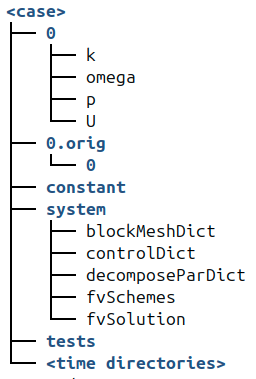
\includegraphics[width=0.33\textwidth]{images/other/OF_arbo.png}
%    \caption{Tree of the OpenFOAM dictionaries}
%    \label{arboOF2}
%\end{figure}


The \texttt{system} directory contains the main parameters regarding the simulation progress:
\begin{itemize}
    \item[$-$] The \texttt{controlDict} dictionary defines parameters such as start and end time, time steps, data output formatting, or data average computation;
    \item[$-$] the \texttt{blockMeshDict} dictionary defines the computational domain, mesh and boundary implementation conditions;
    \item[$-$] the \texttt{decomposeParDict} dictionary defines the geometry and mesh decomposition, with the objective to run the simulation in parallel, using multiple cores;
    \item[$-$] the \texttt{fvSchemes} dictionary defines the discretisation schemes used in the \ac{CPU}s equations;
    \item[$-$] the \texttt{fvSolution} dictionary defines the equation solvers, tolerances and other algorithm controls.
\end{itemize}

The \texttt{constant} directory contains the different physical properties of the simulation. Moreover, the subfolder \texttt{polyMesh} contains the mesh data, obtained after the \texttt{blockMesh} command line is run:
\begin{itemize}
    \item[$-$] The \texttt{momentumTransport} dictionary defines the simulation type (DNS, RANS or LES) and, in the case of RANS or LES, specifies the corresponding turbulence closure or subgrid-scale model.
    \item[$-$] the \texttt{transportProperties} dictionary defines the transport model (e.g., Newtonian) and some transport coefficients, such as the kinematic viscosity $\nu$;
    \item[$-$] the \texttt{MRFProperties} dictionary defined in our case to specify the rotating zone with the origin, rotation axis and rotation speed.
\end{itemize}

The \texttt{0} directory contains the initial solution's fields and the \ac{BC} as well.
A compiled solver can be called in the terminal of the case directory to run the simulation.
If it's called, the \texttt{postProcessing} directory stores data from the running simulation, such as forces and probes' data.
The \texttt{processor0}, ..., \texttt{processor"N-1"} directories directly result from the geometry decomposition, which is proceeded through the \texttt{decomposeParDict} dictionary.
The \texttt{dummy.foam} is an empty file which allows to visualize the simulation with \texttt{ParaView}. 


More precisely, for example, to implement the IBM forcage term on the speed "u", we can manually modify the momentum equation of the corresponding solver as follows:
\begin{lstlisting}[language=C++]
// Momentum predictor step

MRF.correctBoundaryVelocity(U) // Corrects U at boundaries to include MRF effects
                               // (e.g., rotating walls)

tmp<fvVectorMatrix> tUEqn
(
    fvm::div(phi, U)            // Convective term
  + MRF.DDt(U)                  // Time derivative in the rotating reference frame
  + turbulence->ddivDevSigma(U) // Turbulent diffusion term
  + cmptMultiply(Dprime, U - UIB)    // Forcing term: Dprime * (U - UIB)
 ==
    fvModels.source(U)          // Source terms from external models
                                // (e.g., body forces), here equal to 0
);
fvVectorMatrix& UEqn = tUEqn.ref();

UEqn.relax() // Applies under-relaxation for numerical stability

fvConstraints.constrain(UEqn); // Applies physical constraints
                               // (e.g., boundary conditions)
\end{lstlisting}

With
\begin{itemize}
    \item \textit{cmptMultiply} the element-wise matrix multiplication;
    \item $Dprime = \xi \nu D$, with $Dprime$ denoting the reduced form of $D$. The prime symbol is used to distinguish the non-dimensional quantity from its physical counterpart;
    \item $U$ the flow velocity;
    \item $UIB$ is the imposed velocity at the walls. %(here $\Omega \times R$) 
\end{itemize}

%\begin{figure}[H]
%    \centering
%    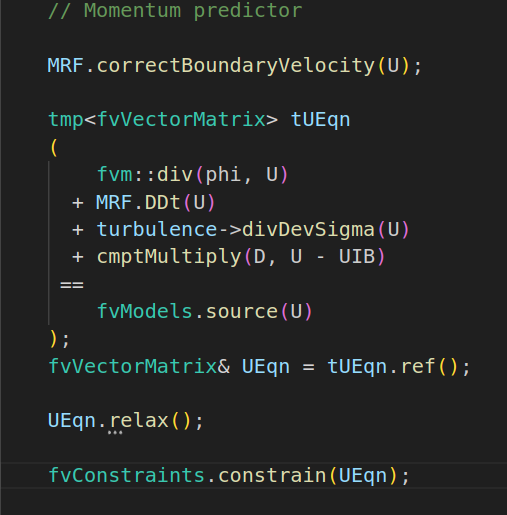
\includegraphics[width=0.5\textwidth]{images/other/implicit_forcing.png}
%    \caption{implicit forcing term in OpenFoam}
%    \label{implicit_forcing}
%\end{figure}


%To compute the time step $\Delta_{t}$ of the pimpleFoam simulation of the pump, we can use the \ac{CFL} condition, which states that:
%\begin{equation}
%    \Delta_{t} = \frac{CFL \cdot \Delta_{x}}{\|U_{\infty}\|},
%\end{equation}
%where: $CFL$ is the Courant number, detail in the \autoref{subsec:CFD_governing_equations}


\subsection{EnKF}
\label{subsec:EnKF}

%\begin{figure}[H]
%    \centering
%    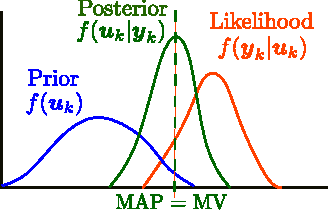
\includegraphics[width=0.33\textwidth]{images/Bayesian_theory.pdf}
%    \caption{Illustration of the Bayesian theorem applied to data assimilation}
%    \label{BayesianTh}
%\end{figure}

As seen in the \autoref{sec:stateOfArt}, we are going to use the stochastic EnKF to assimilate the high-fidelity data.
But first, let's explain the Kalman Filter\footnote{\url{https://cones-dev-pe431-2dbff22738a4d54c2b947e6fa9a9a77fadd187b3bd1a85c.gitlab-pages.ensam.eu/data_assimilation.html}}.

\paragraph{Kalman Filter}

The estimation is calculated by using a set of observations $\mathbf{y}$, a prior state $\mathbf{x}$, and a linear model $\mathbf{M}$. The estimation state is obtained through two operations, the forecast and the analysis, respectively using the superscript \textit{f} and \textit{a}.

The system state $\mathbf{x}_k$ is as follows:
\begin{equation}
\left[
\begin{array}{c}
\mathbf{u}_k \\
\boldsymbol{\theta}_k
\end{array}
\right]
\in \mathbb{R}^{(n_{\text{vars}} \cdot n_{\text{cells}} + n_{\theta}) \times m}
\end{equation}

where:
\begin{itemize}
    \item $\mathbf{u}_k$ is the state matrix (can contain velocities, pressure, temperature...) of the domain at the time instant $k$, which we don't care about in our case;
    \item $\boldsymbol{\theta}_k$ are the model parameters; % coefficients;%, assumed time-invariant in our case;
    \item $m$ is the number of ensemble members.
\end{itemize}

The observation data $\mathbf{y}_k$ is defined as:
\begin{equation}
\left[ \mathbf{y}_k \right]_{n_{\text{obs}}, m} \sim \mathcal{N}(y_k, \mathbf{R}_k)
\end{equation}

Observation data may be built using:
\begin{itemize}
    \item Velocity, pressure, temperature or other physical observed values;
    \item Some discret model parameters such instantaneous global force coefficients $C_D$, $C_L$, $C_f$. In our case, it will be five IBM forcing parameters.
\end{itemize}



\textbf{Prediction step:}
\begin{align}
    \hat{\mathbf{x}}_{k|k-1} &= \mathbf{M}_k \hat{\mathbf{x}}_{k-1|k-1} + \mathbf{B}_k \mathbf{u}_k \\
    \mathbf{P}_{k|k-1} &= \mathbf{M}_k \mathbf{P}_{k-1|k-1} \mathbf{F}_k^\top + \mathbf{Q}_k
\end{align}

\vspace{1em}
\textbf{Update step:}
\begin{align}
    \tilde{\mathbf{y}}_k &= \mathbf{z}_k - \mathbf{H}_k \hat{\mathbf{x}}_{k|k-1} \\
    \mathbf{S}_k &= \mathbf{H}_k \mathbf{P}_{k|k-1} \mathbf{H}_k^\top + \mathbf{R}_k \\
    \mathbf{K}_k &= \mathbf{P}_{k|k-1} \mathbf{H}_k^\top \mathbf{S}_k^{-1} \\
    \hat{\mathbf{x}}_{k|k} &= \hat{\mathbf{x}}_{k|k-1} + \mathbf{K}_k \tilde{\mathbf{y}}_k \\
    \mathbf{P}_{k|k} &= (\mathbf{I} - \mathbf{K}_k \mathbf{H}_k) \mathbf{P}_{k|k-1}
\end{align}

\vspace{1em}
\textbf{Where:}

\begin{multicols}{2}
\setlength{\itemsep}{0pt}
\setlength{\parskip}{0pt}
\begin{itemize}
    \item $\hat{\mathbf{x}}_{k|k-1}$: predicted state at $k$
    \item $\hat{\mathbf{x}}_{k-1|k-1}$: updated state at $k{-}1$
    \item $\mathbf{M}_k$: state transition matrix
    \item $\mathbf{B}_k$: control input matrix
    \item $\mathbf{u}_k$: control input
    \item $\mathbf{P}_{k|k-1}$: predicted covariance
    \item $\mathbf{P}_{k-1|k-1}$: updated covariance at $k{-}1$
    \item $\mathbf{Q}_k$: process noise
    \item $\mathbf{z}_k$: measurement
    \item $\mathbf{H}_k$: observation matrix
    \item $\tilde{\mathbf{y}}_k$: innovation
    \item $\mathbf{S}_k$: innovation covariance
    \item $\mathbf{K}_k$: Kalman gain
    \item $\mathbf{R}_k$: noise measurement
    \item $\mathbf{I}$: identity matrix
    \item $\hat{\mathbf{x}}_{k|k}$: updated state
    \item $\mathbf{P}_{k|k}$: updated covariance
\end{itemize}
\end{multicols}

\begin{figure}[H]
    \centering
    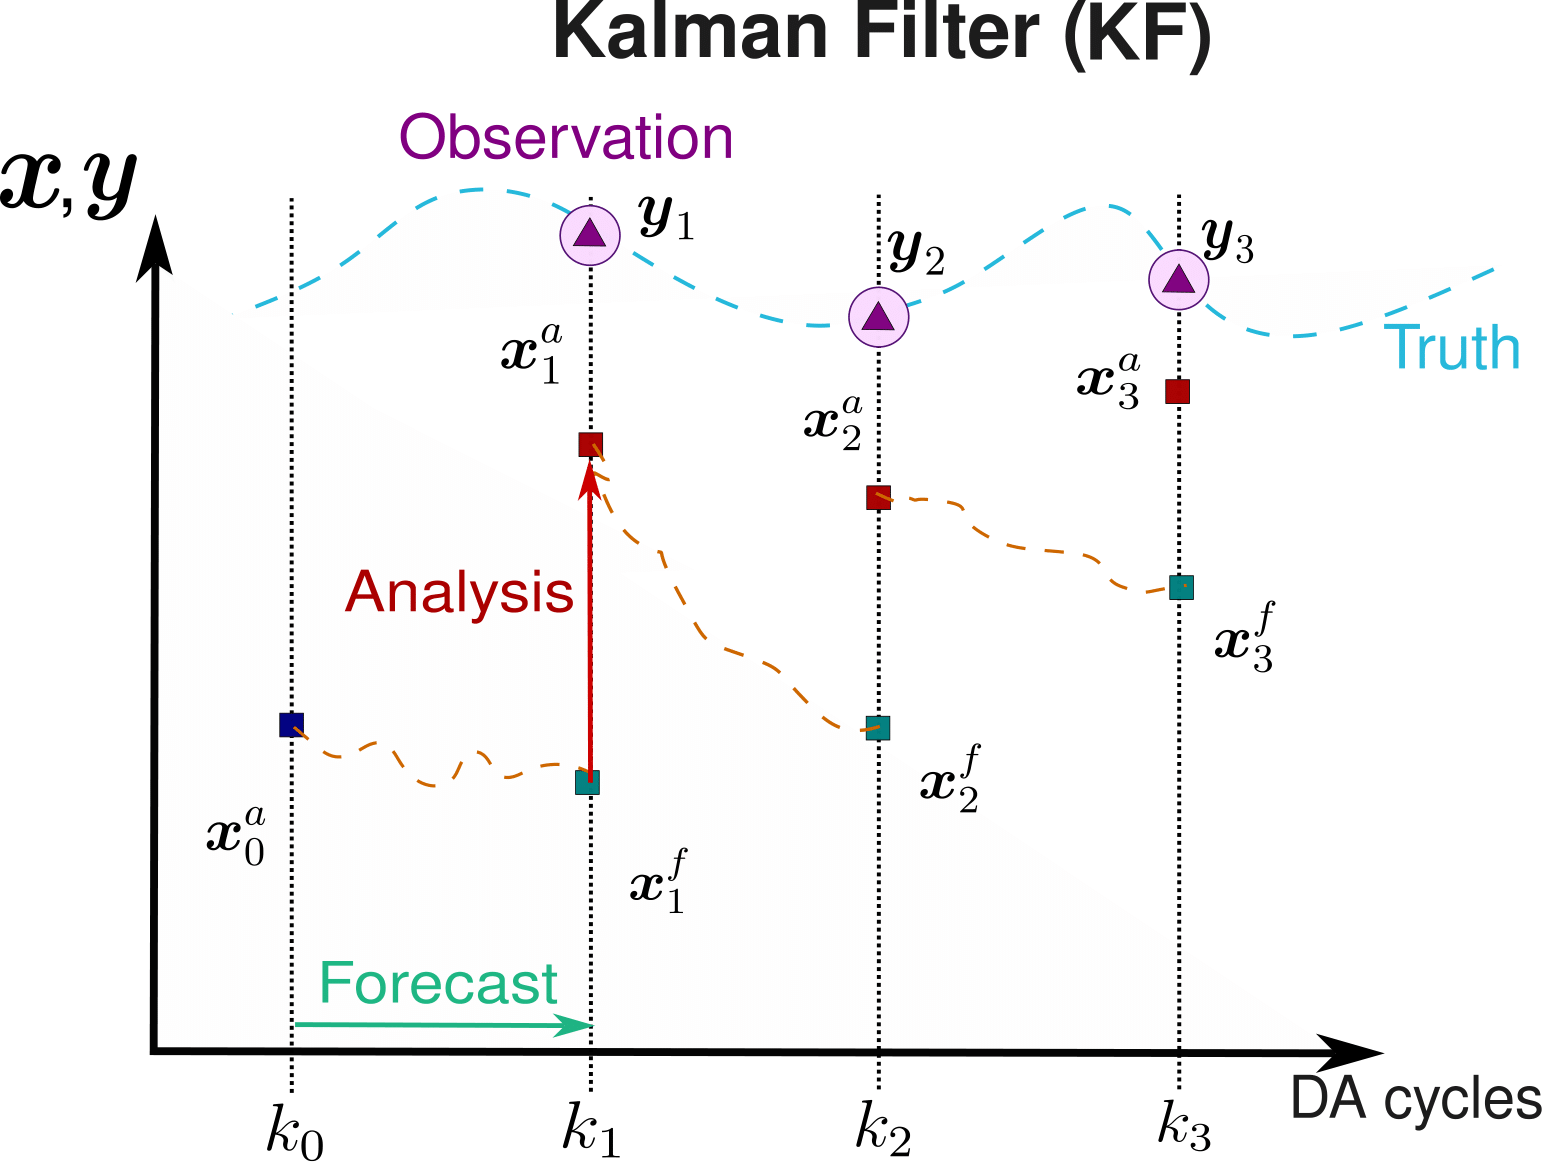
\includegraphics[width=0.7\textwidth]{images/KF_algorithm-1.png}
    \caption{Kalman Filter process illustration}
    \label{KF1}
\end{figure}

Kalman filter presents two main drawbacks that concern our case. First, as the \ac{EKF}, it only works for moderate deviations from linearity and Gaussianity. If $M$ represents the Navier-Stokes equations, then equations are very not linear. Secondly, for a CFD mesh, the covariance matrix $\mathbf{P}_k$ would have a dimention of $(n_{vars} \times n_{cells}, n_{vars} \times n_{cells})$.

The EnKF allows high dimensional systems by avoiding the explicit definition of $\mathbf{P}_k$ and its Monte-Carlo realisations are much more design for non-linear models. A problem can be the underestimation of $\mathbf{P}_k^a$ but the inflation, define later on this subsection, and localisation, helps mitigate this issue.


\begin{comment}
    First \textbf{forecast step (or prediction)} at time \( k \) computes the estimated state \( \mathbf{x}_{k+1}^{f} \) and the error covariance matrix \( \mathbf{P}_{k+1}^{f} \),
\begin{equation}
    \mathbf{x}_{k+1}^{f} = \mathbf{M} \mathbf{x}_k
\end{equation}
\begin{equation}
    \mathbf{P}_{k+1}^{f} = \mathbf{M}_{k+1} \mathbf{P}_k^a \mathbf{M}_{k+1}^\top + \mathbf{Q}
\end{equation}
where \( \mathbf{Q} \) represents the variance matrix of the model.  

Then, the \textbf{analysis step (or correction)} is computed, in which the observation \( \mathbf{y} \) and forecast are combined,
\begin{equation}
    \mathbf{K}_{k+1} = \mathbf{P}_{k+1}^{f} \mathbf{H}^\top \left( \mathbf{H} \mathbf{P}_{k+1}^{f} \mathbf{H}^\top + \mathbf{R}_{k+1} \right)^{-1}
\end{equation}
\begin{equation}
    \mathbf{x}_{k+1}^{a} = \mathbf{x}_{k+1}^{f} + \mathbf{K}_{k+1} \left( \mathbf{y}_{k+1} - \mathbf{H} \mathbf{x}_{k+1}^{f} \right)
\end{equation}
\begin{equation}
    \mathbf{P}_{k+1}^{a} = (\mathbf{I} - \mathbf{K}_{k+1} \mathbf{H}) \mathbf{P}_{k+1}^{f}
\end{equation}
where \( \mathbf{R} \) represents the covariance matrix of the observations, and \( \mathbf{H} \) a linear operator which maps the true state space into the observed space.
\end{comment}



\paragraph{Ensemble Kalman Filter}

We saw previously in this subsection that today, we can theorically run a \ac{DNS} which resolves exactly the Navier-Stokes equations, but it is still too expensive to be used in practice. Therefore, we generally use \ac{LES} or \ac{RANS} models to simulate the flow. The EnKF method can be applied to these models to adjust specific model parameters or flow fields, enhancing the overall physical consistency of the simulation.

A good example based on the simple and academic \textit{cavity test case} illustrates it well.
The cavity test case is a simple flow in a square cavity, where the flow is driven by a moving lid. The flow is characterized by a recirculation zone and a vortex in the center of the cavity. The EnKF method can be used to assimilate data from the flow, such as velocity or pressure measurements, to improve the accuracy of the simulation. The EnKF method can also be used to estimate the parameters of the model, such as viscosity or turbulence model coefficients, to improve the physical accuracy of the simulation.

In our test case, we are going to optimise the velocity wall condition.
To do so, we use the result on 5 locations of a precise converged simulation with a to boundary condition of 5 m.s$^{-1}$ as a reference. We will then assimilate data from the flow, at the 5 observation points (see \autoref{fig:cavity2_1ms}).
We start from a simulation with a wall condition of 1 m.s$^{-1}$, which is not the correct value. The EnKF method will then be used to correct the wall condition by assimilating the data from the flow at the 5 observation points. The EnKF method will iteratively update the wall condition until it converges to the correct value, which is 5 m.s$^{-1}$ in this case. After only three EnKF iterations, the wall condition converges to the correct value (with a relative error of 0.05 m.s$^{-1}$).

\begin{figure}[H]
    \centering
    \begin{subfigure}[b]{0.3\textwidth}
        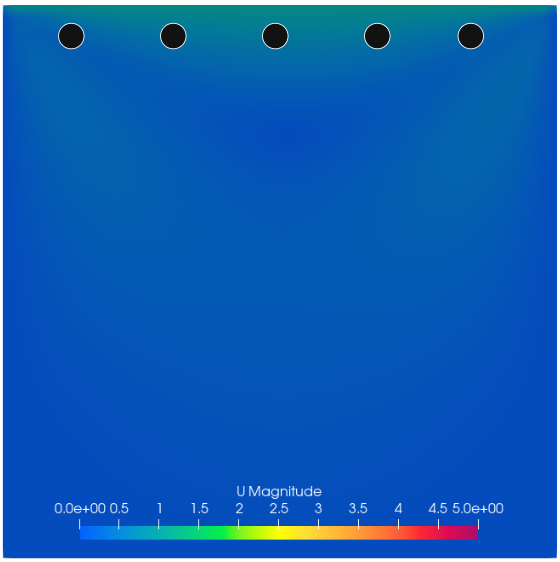
\includegraphics[width=\textwidth]{images/cavity/cavity3_1ms.png}
        \caption{Initial state}
        \label{fig:cavity2_1ms}
    \end{subfigure}
    \hfill
    \begin{subfigure}[b]{0.3\textwidth}
        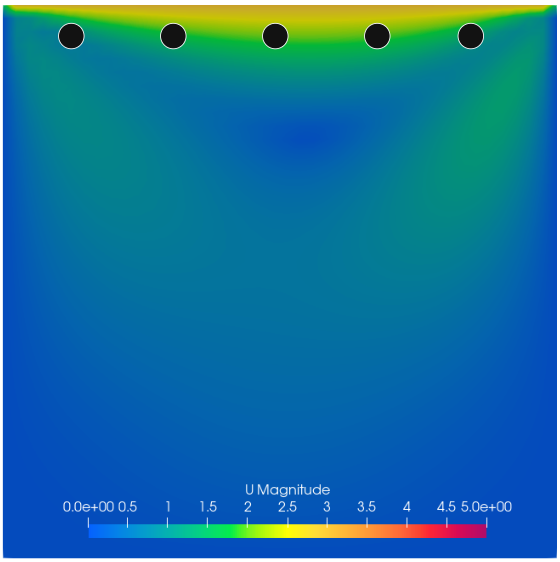
\includegraphics[width=\textwidth]{images/cavity/cavity3_3ms.png}
        \caption{After one EnKF it.}
        \label{fig:cavity2_3ms}
    \end{subfigure}
    \hfill
    \begin{subfigure}[b]{0.3\textwidth}
        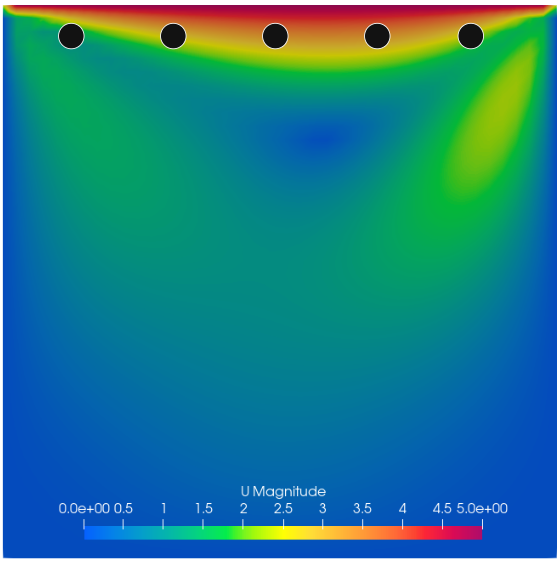
\includegraphics[width=\textwidth]{images/cavity/cavity3_5ms.png}
        \caption{Converged after 2 EnKF it.}
        \label{fig:cavity_5ms}
    \end{subfigure}
    \caption{Evolution of the state through EnKF iterations (
\includegraphics[width=0.013\textwidth]{images/cavity/legende.png}: observation point)}
\end{figure}


The following matrices are needed to build the EnKF algorithm:

\begin{enumerate}
  \item \textbf{Observation covariance matrix} $\mathbf{R}_k$: we assume Gaussian, non-correlated uncertainty for the observations ($\sigma_{i,k}$ is the standard deviation for the variable $i$ at time instant $k$).
  \[
  [\mathbf{R}_k]_{n_{\text{obs}}, n_{\text{obs}}} = \sigma_{i,k}^2 \, [\mathbb{I}]_{n_{\text{obs}}, n_{\text{obs}}}
  \]

  \item \textbf{Sampling matrix} $\mathcal{H} \left( \mathbf{x}_i^f \right)$: it is the projection of the model into the position of the observations.
  \[
  \left[ \mathcal{H} \left( \mathbf{x}_i^f \right) \right]_{n_{\text{obs}}, m}
  \]

  \item \textbf{Anomaly matrices} for the system’s state $\mathbf{x}_i^f$ and sampling $\mathcal{H} \left( \mathbf{x}_i^f \right) = \mathbf{s}_i^f$ matrices. They measure the deviation of each realization with respect to the mean.
  \[
  \mathbf{X}_i = \frac{\mathbf{x}_i - \bar{\mathbf{x}}}{\sqrt{m-1}}, \quad 
  \mathbf{S}_i = \frac{\mathbf{s}_i - \bar{\mathbf{s}}}{\sqrt{m-1}}
  \]
  with
  \[
  [\mathbf{X}]_{n_{\text{vars}} \times (n_{\text{cells}} + n_{\theta}), m}, \quad 
  [\mathbf{S}]_{n_{\text{obs}}, m}
  \]

  \item \textbf{Kalman Gain matrix}:
  \[
  \mathbf{K} = \mathbf{X} \mathbf{S}^\top \left( \mathbf{S} \mathbf{S}^\top + \mathbf{R} \right)^{-1}
  \]
  with
  \[
  [\mathbf{K}_k]_{n_{\text{vars}} \times (n_{\text{cells}} + n_{\theta}), n_{\text{obs}}}
  \]
\end{enumerate}





%$\mathcal{M}$ (model), $\boldsymbol{R}$ (observation covariance), $\boldsymbol{y}_k$ (observations),\\
%$\boldsymbol{u}_{i,0}^\prime = [\boldsymbol{u}_{i,0}, \theta_{i,0}]^T$ (initial states with $\boldsymbol{u}_{i,0} \sim \mathcal{N}(\boldsymbol{\overline{u}}_0, \boldsymbol{P}_0)$ and $\theta_{i,0} \sim \mathcal{N}(\overline{\theta}_0, \boldsymbol{P}_0)$)


For RANS representation, there is no physical time advancement of the model, so each instant is represented through a different interation of the solver.%, and 

\begin{algorithm}[!ht]
    \caption{Scheme of the EnKF used in the present analyses for parameter optimization.}
    \label{alg:EnKF}
    \begin{algorithmic}[1]
        \State \textbf{Input:} $\mathcal{M}$ (model); $\boldsymbol{R}$ (observation covariance); $\boldsymbol{y}_k$ (observations);

        %$\boldsymbol{u}_{i,0}^\prime = [\boldsymbol{u}_{i,0}, \theta_{i,0}]^T$ (initial prior states with $\boldsymbol{u}_{i,0} \sim \mathcal{N}(\boldsymbol{\overline{u}}_0, \boldsymbol{P}_0)$ and $\theta_{i,0} \sim \mathcal{N}(\overline{\theta}_0, \boldsymbol{P}_0)$)
        $\boldsymbol{x}_{i,0} = [\boldsymbol{u}_{i,0}, \theta_{i,0}]^T$ (initial prior states with $\boldsymbol{u}_{i,0} \sim \mathcal{N}(\boldsymbol{\overline{u}}_0, \boldsymbol{P}_0)$ and $\theta_{i,0} \sim \mathcal{N}(\overline{\theta}_0, \boldsymbol{P}_0)$)

        $k = 1, 2, ..., K$ is the iteration index; $i = 1, 2, ..., N_e$ is the ensemble index

        \For{$k = 1$ to $K$}
            \For{$i = 1$ to $N_e$}
                \State Advance in time: $\boldsymbol{u}_{i,k}^f = \mathcal{M}(\theta_{i,k-1})\,\boldsymbol{u}_{i,k-1}$
                \State Observation: $\boldsymbol{Y}_{i,k} = \boldsymbol{y}_k + \boldsymbol{e}_i$, $\boldsymbol{e}_i \sim \mathcal{N}(0,\boldsymbol{R})$
                %\State Compute ensemble means: $\boldsymbol{\overline{u}}_k^{\prime^f} = \frac{1}{N_e}\sum_{i=1}^{N_e}\boldsymbol{u}_{i,k}^{\prime^f}, \overline{\mathcal{H}(\boldsymbol{u}^f_k}) = \frac{1}{N_e}\sum_{i = 1}^{N_e} \mathcal{H}(\boldsymbol{u}_{i,k}^f)$
                \State Predicted observation: $s_{i,k} = \mathcal{H}(\boldsymbol{u}_{i,k}^f)$
                \State Ensemble means: $\boldsymbol{\overline{x}}_k^{f} = \frac{1}{N_e}\sum_{i=1}^{N_e}\boldsymbol{x}_{i,k}^{f}, \overline{s_{i,k}} = \frac{1}{N_e}\sum_{i = 1}^{N_e} s_{i,k}$
                %\State Anomaly matrices: $\boldsymbol{X}_k = \frac{\boldsymbol{u}_{i,k}^{\prime^f} - \boldsymbol{\overline{u}}_k^{\prime^f}}{\sqrt{N_e - 1}}$,\,$\boldsymbol{S}_k = \frac{\mathcal{H}(\boldsymbol{u}_{i,k}^f) - \overline{\mathcal{H}(\boldsymbol{u}^f_k)}}{\sqrt{N_e-1}}$
                \State Anomaly matrices: $\boldsymbol{X}_k = \frac{\boldsymbol{x}_{i,k}^{f} - \boldsymbol{\overline{x}}_k^{f}}{\sqrt{N_e - 1}}$,\,$\boldsymbol{S}_k = \frac{s_{i,k} - \overline{s_{i,k}}}{\sqrt{N_e-1}}$
                \State Kalman gain: $\boldsymbol{K}_k = \boldsymbol{X}_k^f(\boldsymbol{S}_k)^T [\boldsymbol{S}_k(\boldsymbol{S}_k)^T + \boldsymbol{R}]^{-1}$ % \boldsymbol{L} \odot 
                %\State Update: $\boldsymbol{u}_{i,k}^{\prime^a} = \boldsymbol{u}_{i,k}^{\prime^f} + \boldsymbol{K}_k (\boldsymbol{Y}_{i,k} - \mathcal{H}(\boldsymbol{u}_{i,k}^f))$
                \State Update: $\boldsymbol{x}_{i,k}^{a} = \boldsymbol{x}_{i,k}^{f} + \boldsymbol{K}_k (\boldsymbol{Y}_{i,k} - \mathcal{H}(\boldsymbol{u}_{i,k}^f))$
                %\State (Deterministic) covariance inflation: $\boldsymbol{u}_{i,k}^{\prime^a} = \boldsymbol{\overline{u}}_k^{\prime^a} + \lambda_k (\boldsymbol{u}_{i,k}^{\prime^a} - \boldsymbol{\overline{u}}_k^{\prime^a})$
                \State (Deterministic) covariance inflation: $\boldsymbol{x}_{i,k}^{a} = \boldsymbol{\overline{x}}_k^{a} + \lambda_k (\boldsymbol{x}_{i,k}^{a} - \boldsymbol{\overline{x}}_k^{a})$
            \EndFor
        \EndFor
    \end{algorithmic}
\end{algorithm}

Observation data $y$ can be some local sensors (such as PIV data) or global variables (such as performance)

With $\boldsymbol{\overline{x}}_k^{f} = [\boldsymbol{\overline{u}}_k^f, \overline{\theta}_{k-1}]^T$ and $\boldsymbol{x}_{i,k}^{f} = [\boldsymbol{u}_{i,k}^f, \theta_{i, k-1}]^T$


In our case, $\boldsymbol{\overline{x}}_k^{f} = [\overline{\theta}_{k-1}]^T$, $\boldsymbol{x}_{i,k}^{f} = [\theta_{i, k-1}]^T$, $\lambda_k = 0$ and $\boldsymbol{y}_k = \boldsymbol{y}$.



Some \textit{deterministic inflation} is included to increase the variability of the state predicted by the EnKF:

\begin{equation}
    \boldsymbol{\alpha}_{i,k}^a = \boldsymbol{\overline{\alpha}}_k^a + \lambda_k \left(\boldsymbol{\alpha}_{i,k}^a - \boldsymbol{\overline{\alpha}}_k^a   \right)
    \label{eqn:inflation}
\end{equation}

where $\boldsymbol{\alpha}$ can be either the state vector $\boldsymbol{u}$ or the model parameters $\theta$.

Here is an illustration of the deterministic inflation, that increase the variability of the member ensemble to avoid a too fast collaps and permit to have more chance to find a lower local (or in a better case, global) minimum solution:
\begin{figure}[H]
    \centering
    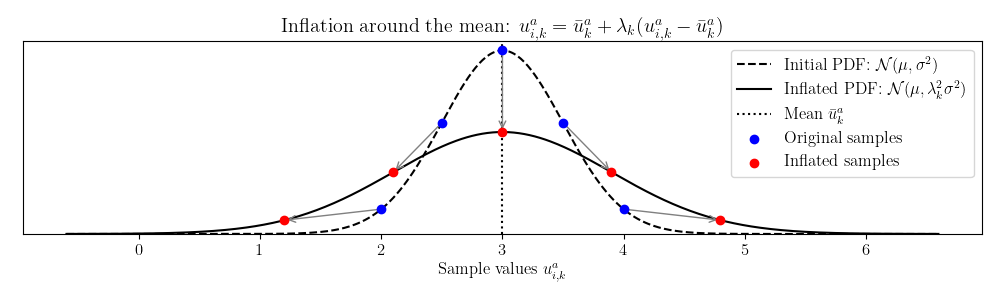
\includegraphics[width=1\textwidth]{images/inflation.png}
    \caption{Deterministic inflation}
    \label{fig:inflation}
\end{figure}

I coded it but it finally was not needed for the centrifugal pump case.

\begin{comment}
\begin{algorithm}[h!]
    \caption{Scheme of the EnKF used in the present analyses for both state estimation and parameter optimization.}
    \label{alg:EnKF}
    \KwIn{$\mathcal{M}$ (model), $\boldsymbol{R}$ (observation covariance), $\boldsymbol{y}_k$ (observations),\\
    \qquad $\boldsymbol{u}_{i,0}^\prime = [\boldsymbol{u}_{i,0}, \theta_{i,0}]^T$ (initial states with $\boldsymbol{u}_{i,0} \sim \mathcal{N}(\boldsymbol{\overline{u}}_0, \boldsymbol{P}_0)$ and $\theta_{i,0} \sim \mathcal{N}(\overline{\theta}_0, \boldsymbol{P}_0)$)}
    \KwData{$k = 1, 2, ..., K$ is the iteration index; $i = 1, 2, ..., N_e$ is the ensemble index}
    \For{$k \leftarrow 1$ \KwTo $K$}{
        \For{$i \leftarrow 1$ \KwTo $N_e$}{
            \nl Advancement in time of the state vectors:\;
            \qquad $\boldsymbol{u}_{i,k}^f = \mathcal{M}(\theta_{i,k-1})\,\boldsymbol{u}_{i,k-1}$\;
            \nl Generation of an observation matrix from the confidence level:\;
            \qquad $\boldsymbol{Y}_{i,k} = \boldsymbol{y}_k + \boldsymbol{e}_i$, where $\boldsymbol{e}_i \sim \mathcal{N}(0,\boldsymbol{R})$\;
            \nl Estimation of the ensemble means:\;
            \qquad $\boldsymbol{\overline{u}}_k^{\prime^f} = \frac{1}{N_e}\sum_{i=1}^{N_e} \boldsymbol{u}_{i,k}^{\prime^f}$,\;
            \qquad $\overline{\mathcal{H}(\boldsymbol{u}_k^f)} = \frac{1}{N_e} \sum_{i=1}^{N_e} \mathcal{H}(\boldsymbol{u}_{i,k}^f)$\;
            \nl Compute anomalies:\;
            \qquad $\boldsymbol{X}_k = \frac{\boldsymbol{u}_{i,k}^{\prime^f} - \boldsymbol{\overline{u}}_k^{\prime^f}}{\sqrt{N_e - 1}}$,\;
            \qquad $\boldsymbol{S}_k = \frac{\mathcal{H}(\boldsymbol{u}_{i,k}^f) - \overline{\mathcal{H}(\boldsymbol{u}_k^f)}}{\sqrt{N_e - 1}}$\;
            \nl Kalman gain with localisation:\;
            \qquad $\boldsymbol{K}_k = \boldsymbol{L} \odot \boldsymbol{X}_k (\boldsymbol{S}_k)^T \left[\boldsymbol{S}_k (\boldsymbol{S}_k)^T + \boldsymbol{R}\right]^{-1}$\;
            \nl Update state matrix:\;
            \qquad $\boldsymbol{u}_{i,k}^{\prime^a} = \boldsymbol{u}_{i,k}^{\prime^f} + \boldsymbol{K}_k \left(\boldsymbol{Y}_{i,k} - \mathcal{H}(\boldsymbol{u}_{i,k}^f)\right)$\;
            \nl Deterministic covariance inflation:\;
            \qquad $\boldsymbol{u}_{i,k}^{\prime^a} = \boldsymbol{\overline{u}}_k^{\prime^a} + \lambda_k \left(\boldsymbol{u}_{i,k}^{\prime^a} - \boldsymbol{\overline{u}}_k^{\prime^a}\right)$\;}}
\end{algorithm}
\end{comment}



\subsection{The CONES library}
CONES is a library coded in Python/C++, that has been developed since 2022 at LMFL. % stands for "Coupling OpenFOAM with Numerical EnvironmentS" and
It is the only code that permits online DA in CFD codes (it uses \ac{MPI} process to do it).
It's parallelized and can be used on supercomputers. It is mainly designed to work with OpenFOAM and DA codes as EnKF.\label{instants_partages}


A specific directory structure must be observed, as outlined in \autoref{fig:CONES}.
Let's take our OpenFOAM/EnKF example as support to explain CONES. Concretly, on one side, $m$ OpenFOAM simulations are running with run at the same time on $n$ processors and on the other side, the EnKF runs on $e$ processors (usually only one is enough).
At the begining, all variables are initialized on both sides, using MPI process.
Then, all simulation run at same time (with different initial states).
Sampled data ($H(u_k^f)$) and 
$
    \left[
    \begin{array}{c}
    \mathbf{u}_k \\
    \boldsymbol{\theta_k}
    \end{array}
    \right]^f
$
are send to the EnKF. Using $y_k$, EnKF algorithm can compute and send back the updated velocity field (not computed in our case) and the parameters $\theta_k^a$ to the different ensemble members (each are different befor converging).
With these new parameters, the loop can be done again.

% \autoref{fig:OpenFOAM_directory_structure}:
% décrire la structure du dossier OpenFOAM et ce que chaque fichier fait (dans mon cas de simulation)

\begin{figure}[H]
    \centering
    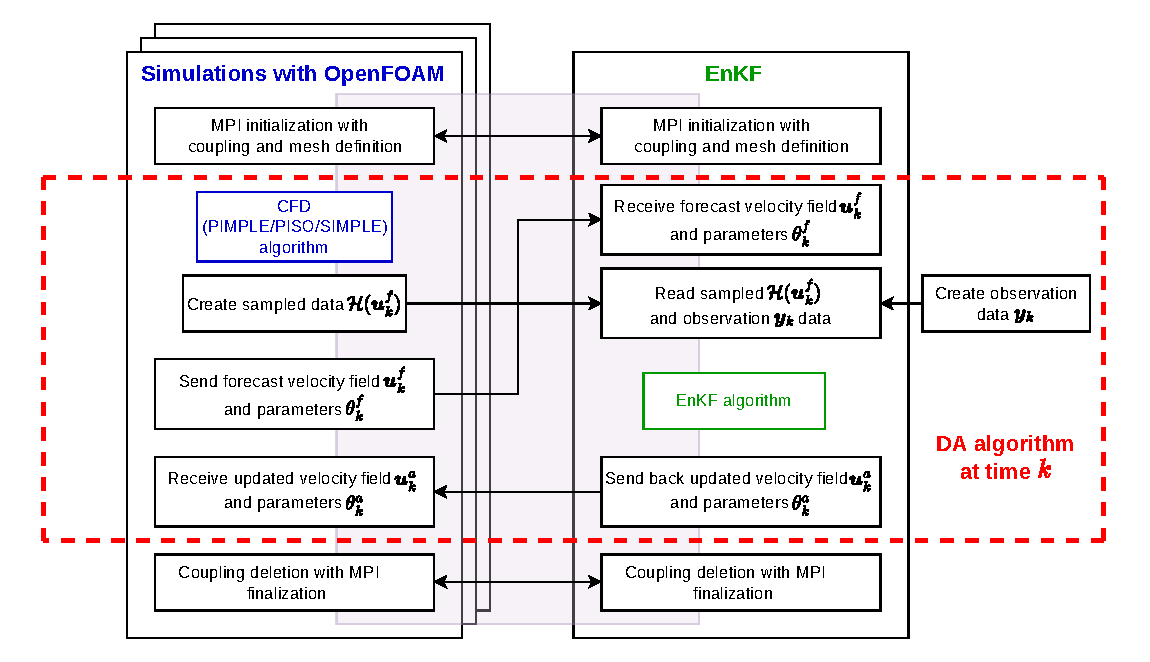
\includegraphics[width=1\textwidth]{images/EnKF_ConesWithouCWIPI.pdf}
    \caption{CONES structure}
    \label{fig:CONES}
\end{figure}


